\documentclass[11pt,a4paper]{report}
\usepackage[latin1]{inputenc}
\usepackage{amsmath}
\usepackage{amsfonts}
\usepackage{amssymb}
\usepackage{graphicx}
\usepackage[left=3.00cm]{geometry}
\usepackage{pdfpages}
\linespread{1.25}
\usepackage{helvet} %uarial alt. package for arial font! Try to see if its better
\usepackage{natbib} %https://www.sharelatex.com/learn/Natbib_citation_styles
\usepackage{Appendix}
\usepackage[none]{hyphenat}
\renewcommand{\familydefault}{\sfdefault}

\title{An Investigation into the Real World Impact of Robot Affect through Speech and Movement}
\author{Katie Winkle}
\date{A dissertation submitted in partial fulfilment of the requirements of the University of the West of England, Bristol and of the University of Bristol for completion of the first stage of the FARSCOPE Doctor of Philosophy Programme 
\newline 
\newline
Module Number : UFMFRG-80-M (EMATM0020) 
\newline 
\newline
Faculty of Engineering Technology, University of the West of England, Bristol
\newline
\newline
September 2016}
\begin{document}
\maketitle

\section*{Declaration}
This study was completed as part of the FARSCOPE Centre for Doctoral Training at the University of Bristol and the University of the West of England, Bristol.  The work is my own.  Where the work of others is used or drawn on it is attributed.
\newline
\newline
\newline
\newline
\_\_\_\_\_\_\_\_\_\_\_\_\_\_\_\_\_\_\_\_\_\_\_\_\_\_\_\_\_\_\_\_\_\_\_\_\_\_\_\_\_\_\_\_
\newline
\newline
Katie Winkle
\newline
\newline
\newline
Word Count: 12,088 Words

\newpage
\section*{Abstract}

Interpersonal emotion transfer (IET) is a psychological phenomenon observed in humans concerning the sharing of emotions between persons and its consequences. One observed form of IET is emotion contagion, in which one person `catches' the emotion of another. Another is social appraisal, where one person's judgement of something is affected by the emotional response of another \cite{parkinson2011interpersonal}. The overall aim of this project is to investigate the real world potential of robot to human IET and emotional expression in human robot interaction (HRI). 

Emotional expression was implemented on Softbank Robotics' NAO robot using an implementation of Lim et al.'s SIRE parameterisation framework for gesturing \cite{lim2011converting} and CereProc's Cerevoice Text-to-Speech SDK with built-in emotion support for speech. A HRI experiment consisting of a robot-led arm exercise session was undertaken in order to address the main project aim within a real-world application context. 

Participants in the exercise session experiment failed to recognise the robot's intended emotional state. This contrasts with good emotion recognition results achieved in validation of the system. Likely due to this lack of recognition, no significant differences in participants' behaviour or responses were found across the different emotional conditions. A key conclusion from this work is that emotion portrayal through robot voice and gesture may only be possible if users witness different emotional conditions, therefore seeing a difference in robot behaviour which can be associated with a changing emotional state.

\newpage
\section*{Acknowledgements}
I would first like to thank my supervisor Dr Paul Bremner for consistently allowing this work to be my own whilst providing the support and guidance to bring it to fruition. I would also like to thank Dr Praminda Caleb-Solly for her valuable insight into the area of assisted living robotics and interesting discussions on future applications of my research. Finally I would like to thank all of my colleagues at the Bristol Robotics Laboratory, the University of Bristol and the University of the West England who answered my many calls for experiment participants and pilot testers; I couldn't have produced this work without your willing participation.
\newline
\newline
This work was supported by the EPSRC Centre for Doctoral Training in Future Autonomous and Robotic Systems (FARSCOPE) at the Bristol Robotics Laboratory.

\tableofcontents

\chapter{Introduction}
Social robotics looks to equip robots with human-like social intelligence in order to provide natural and intuitive interactions which move ever more towards emulating human-human interaction (HHI) \cite{breazeal2004designing}. Typically this has involved utilising human communication behaviours such as gesturing \cite{bremner2011effects}, eye contact and gaze direction \cite{chidambaram2012designing}. In the field of socially assistive robotics, social robots are being employed in increasingly emotionally delicate situations, for example as social companions in long term care facilities \cite{louie2012playing} or as playmates for children \cite{tielman2014adaptive}. As such, there is an increasing amount of interest in robots that can portray human-like emotions and the impact this can have on human robot interaction (HRI) (e.g. \cite{Angeli2014}, \cite{xu2014robot},  \cite{kim2010designing}).

\section{Motivation}
Human beings naturally utilise affective communication behaviours such as facial expression, body posturing and gesturing in order to effectively communicate their emotional state. On a subconscious level emotions play an important part in human interaction; they affect the judgements we make and guide our actions. Additionally we seem to be able to `catch' each others emotions; we feel down when our friends are down and we might try to cheer them up by being cheerful ourselves. These effects can be grouped together under the term interpersonal emotion transfer (IET). \cite{parkinson2011interpersonal}. 

The psychological phenomenon of IET between humans is still not fully understood; however, it is believed to include social appraisal and emotion contagion effects \cite{parkinson2011interpersonal}. In this context social appraisal describes a person's judgement of something being affected by the emotional response of another (i.e. affecting what they think), whereas emotion contagion describes a change in their emotional state (i.e. affecting how they feel). For example, it has been demonstrated that listening to a neutral text spoken happily or sadly can induce similar feelings in the listener \cite{neumann2000mood} and that the same household object will be rated differently if it is presented alongside a picture of a smiling or disgusted face \cite{bayliss2007affective}. In addition, there is growing evidence that nonverbal emotional expression is an important and subconscious part of human communication which has evolved as a mechanism for quickly communicating a range of information such as social status and level of threat (see \cite{tracy2015nonverbal} for a review). 

Based on this there are at least two major reasons for wanting to design a robot with IET capabilities. Firstly, if emotional expression is an important part of human communication, then a robot with such capabilities might be more lifelike, more likeable and more natural to interact with. Secondly, the effects of IET described above, e.g shaping people's judgement or decision making and impacting on how they feel, might be beneficial in a range of HRI applications just as it is in HHI. Some example HRI scenarios where emotional expression might be useful follow directly from those demonstrated in HHI, e.g. in collaborative team-working \cite{barsade2002ripple} or maintaining calm \cite{latane1968group}. Arguably however the biggest potential application of robot to human IET is in the growing area of socially assistive robotics \cite{feil2005defining}. Socially assistive robots provide users with non-physical assistance generally through a companionship style relationship. Demonstrated examples include a weight loss coach for the home \cite{kidd2008robots}, a memory game playing robot for long term care facilities \cite{louie2012playing}, a companion robot for maintaining older adults' independence \cite{nani2010mobiserv}, a robot exercise instructor \cite{fasola2010robot} and a robot language tutor \cite{kennedy2016social}. Endowing such robots with IET capabilities might offer the following functionality benefits: 
\begin{itemize}
	\item The robot could provide more realistic and enjoyable social companionship
	\item The robot could `cheer up' the user by being cheerful itself
	\item The robot could give the user a positive impression of potentially undesirable tasks, e.g. taking medication or doing exercise
	\item The robot could provide more effective encouragement during activities like those above
	\item The robot could appear empathetic and caring, leading to a better human-robot relationship
\end{itemize}

However, this reasoning assumes that IET occurs equally well in HRI as in HHI and that the effects demonstrated in the psychology literature could be triggered by robots in the same way as by humans. Arguably, given the well known effect of the `uncanny valley' \cite{mori2012uncanny}, this assumption might not be valid and hence warrants further study. Research done so far suggest demonstrates that recognisable emotional expression is certainly possible in a range of robots (e.g.\cite{masuda2009emotion}, \cite{lim2011converting}, \cite{tielman2014adaptive}), however the impact of this on a human's own emotional state and the robot's effectiveness is less well documented. 

Many robots either commercially available or utilised in research do not have adaptable facial expression. A 2016 business review of commercially available personal robots contained five such robots \cite{sweet2016} including the Pepper robot; designed foremost to be an emotional robot companion\footnote{https://www.ald.softbankrobotics.com/en/cool-robots/pepper}. These are shown in Figure \ref{fig:socialRobots}. Looking further afield and considering assistive robots more generally, additional examples of robots without facial expression capabilities can be found,e.g. the MOBISERV service robot companion\footnote{http://www.mobiserv.info/}. Assistive robots by definition provide some level of assistance to the user and therefore have functional requirements which must be met in order for the robot to be effective. For this reason it is desirable that any emotion expression framework is generic and can be applied to functional tasks rather than requiring specific semantic motions or utterances. 

\begin{figure}
\centering
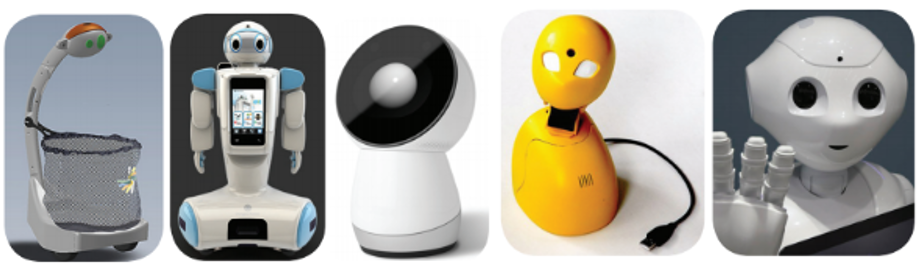
\includegraphics[width=\linewidth]{socialRobots}
\caption{A selection of commercially available personal robots lacking facial expression capabilities \cite{sweet2016}. From left to right: Budgee by 5elementsrobotics, Hovis Genie by DST Robot, Jibo by Jibo, OriHime by Ory  and Pepper by SoftBank Robotics}
\label{fig:socialRobots}
\end{figure}


\section{Problem Statement}

The potential benefits of robot emotional expression and robot to human IET are clear. However, there is still significant uncertainty and a lack of evidence concerning whether IET from a robot to a human can occur  and, if so, what impact this might have on the robot's effectiveness and/or the human's task performance. This project aims to address this uncertainty and lack of evidence in order to evaluate the real world potential of robot-human IET. Based on contextualising the investigation in terms of real world applications, only generic, semantic-free emotion expression methods using voice and motion will be considered. Softbank Robotics' humanoid robot NAO\footnote{https://www.aldebaran.com/en/cool-robots/nao} was chosen to be the robot platform used for this project in line with previous work investigating robot emotion through voice and gesture \cite{lim2011converting} \cite{xu2013mood}. 

\section{Aims and Objectives}
\subsection{Aims}
The overall aim of this project is to investigate the real world potential of emotional expression through voice and gesture in robot to human communication.  This can be broken down into three key project aims:

\begin{enumerate}
	\item Investigate robot to human emotion transfer through robot voice and gesture
	\item Investigate the impact of affective robot communication on HRI
	\item Contextualise all investigations with reference to real world robot applications 
\end{enumerate}

The first aim deals specifically with exploring emotion transfer, i.e. whether a human's emotional state can be changed through interaction with a robot demonstrating emotionally valenced movements and speech. The second aim is to explore, regardless of whether emotion transfer occurs, how such emotional expression might impact on HRI. Some aspects for consideration are listed under Objective 3, however defining specific evaluation measures is non-trivial and makes up part of the required investigation. Generally it is the impact on the robot's effectiveness that should be considered; however the definition of effectiveness depends on the purpose of the robot. This feeds into the final aim to contextualise all investigations with reference to current robotics trends and likely future applications in which the potential benefits of robot to human IET might be desirable. 

\subsection{Objectives}
In order to achieve the project aims, a list of specific objectives was derived as follows: 
\begin{enumerate}
	\item Study affective communication and emotion contagion
	\begin{itemize}
		\item Specifically consider semantic free voice and motion emotional expression
		\item Consider the role emotion contagion plays in HHI
	\end{itemize}
	\item Implement a method for generating emotional robot expression on the NAO platform
	\begin{itemize}
		\item Method(s) should be generic e.g. a parameter based framework
		\item Conduct evaluation experiment(s) for method refinement
	\end{itemize}
	\item Conduct contextualised HRI experiment(s) to test the impact of affective robot communication
	\begin{itemize}
		\item Base experiment contextualisation on real world applications of social robots
		\item Consider human behaviour, emotional state and perception of the robot
		\item Implement appropriate experimental measures covering the above considerations
	\end{itemize}
\end{enumerate}

\section{Work Summary}
The literature review presented in Chapter 2 covers three key areas; IET and emotional expression in humans, emotional expression in robots and experimentally evaluating the impact of robot affect. The first section deals with understanding how humans portray emotion and what consequences that can have on HHI, human behaviour and emotional state. The second section discusses previous work in making robots appear emotional through the use of movement and voice. Specifically this is focused on parameter-based frameworks that can be applied to functional gestures or neutral speech rather than requiring specific semantic demonstrations. The final section considers previous HRI studies considering affective communication or other elements of robot behaviour; these provide inspiration for experiment design and experimental measures.

The research methodology presented in Chapter 3 describes how emotional expressions were generated on the NAO, how these expressions were validated and design of the main experiment used to test the impact of affective robot communication on HRI. Emotion expression on the NAO was done using an implementation of Lim et al.'s SIRE parameterisation framework for gesturing \cite{lim2011converting} and CereProc's Cerevoice Text-to-Speech SDK\footnote{https://www.cereproc.com/en/products/sdk} with built-in emotion support for speech. This was validated using online emotion recognition surveys considering gesture only, voice only and voice and gesture combined. A robot-led arm exercise session context was chosen for the main HRI experiment with a wide range of experimental measures covering human motivation, engagement, enjoyment and perception of the robot. 

The results of the exercise session experiment are presented in Chapter 4 and discussed in Chapter 5. Emotion recognition was high in the validation experiments but was not achieved in the exercise session. This is likely due to the between-subject experiment design; previous work considering robot emotion through voice and gesture and the validation experiments undertaken in this project utilised within-subject testing. Additional analysis of the validation results yielded the interesting observation that the use of gestures seems to increase the perceived extremity of the robots emotional state. Results from the exercise session experiment suggest that the addition of affective communication had very little impact on participants; however this is likely due to the lack of emotion recognition described previously. 

Conclusions based on these results and discussion are provided in Chapter 6 along with recommendations for further investigations and a note on the limitations of this work. Most notable is the conclusion that portraying robot emotion through voice and gesture only may only be possible if the user witnesses the robot in different emotional conditions, such that they can see the difference in the robot's behaviour. This has implications for portraying emotion using voice and gesture in robots that are likely to be interacted with infrequently or on single occasions by different rather than repeat users. 

\chapter{Literature Review}
The literature review presented here covers three key areas; interpersonal emotion transfer (IET) and emotional expression in humans, emotional expression in robots and experimentally evaluating the impact of robot affect. The first section deals with understanding how humans portray emotion and what consequences that can have on human-human interaction (HHI), human behaviour and emotional state. The second section discusses previous work in making robots appear emotional through the use of movement and voice. Specifically this is focused on parameter-based frameworks that can be applied to functional gestures or neutral speech rather than requiring specific semantic demonstrations. The final section considers previous human robot interaction (HRI) studies considering affective communication or other elements of robot behaviour; these provide inspiration for experiment design and experimental measures.

\section{IET and Emotional Expression in Humans}

\subsection{IET and its Impact on Human Behaviour}
There are different hypotheses concerning the purpose of IET and emotional expression more generally in HHI. A functionalist approach (considering the consequences in order to determine the purpose) suggests that at the dyadic level, emotion expressions help individuals determine others' emotions, beliefs, intentions and orientation towards their relationship; and that evoking emotions in others is associated with behaviours such as avoidance, helping, affiliation and soothing \cite{keltner1999social}. An evolutionary approach (considering development over time and the link to population fitness) suggests that emotional expression evolved from being a physiological response (e.g. scrunching the nose to prevent inhalation of noxious gas) into a form of social communication, which observers evolved an ability to instantly and subconsciously decode in order to obtain information about the expresser and/or their environment \cite{shariff2011emotion}. Regardless of exact purpose, a consistent theme in psychology literature is the importance and subconscious nature of IET resulting from emotional expression in communication, and this is what has the greatest relevance to HRI. 

There is evidence to suggest that one form of IET is social appraisal, whereby individual human judgement is influenced by the perceived judgement of others \cite{parkinson2011interpersonal}. Specifically, it has been demonstrated that judgement of an everyday object differs depending on whether it is presented alongside a smiling or disgusted face \cite{bayliss2007affective} suggesting that emotional expression is a trigger for this form of IET. Another experiment demonstrated that even in a very dangerous situation (a simulated fire) participants surrounded by seemingly calm and unresponsive actors were slower to react than participants that were alone; it has been argued that this could be due to IET effects whereby the participants felt calmer due to the calmness of the actors and also judged the situation to be less dangerous based on their perceived lack of concern (\cite{latane1968group} as discussed in \cite{parkinson2011interpersonal}).

Another evidenced form of IET is emotion contagion, whereby an individual's emotional state changes based on that of their interaction partner; however, this is less well understood and more difficult to experimentally examine than social appraisal effects \cite{parkinson2011interpersonal}. There is a general consensus that most emotion contagion is a form of social mimicry, however, it is disputed whether this is based on physical mimicry, in which the related emotion is generated from mimicking the physical expression; i.e. the individual smiles in response to a smile and hence feels happier \cite{strack1988inhibiting}, or whether expression is less important and actually an individual must understand and perceive the reason for another's emotional expression in order for emotion contagion to occur \cite{tamietto2009unseen}. Physical mimicry may not actually be required, for example listening to neutral information spoken in an emotional way can induce similar emotions in the listener \cite{neumann2000mood}. In contrast to the idea of simple mimicry it should also be noted that emotion contagion has been demonstrated to induce contrasting as well as than matching emotions, and that this may be linked to social stature \cite{tiedens2003power}.

Demonstrated examples of emotion contagion highlight the impact it can have both at the individual and group level. For example, contagion of happiness or anger can increase or decrease trust respectively \cite{dunn2005feeling} and emotion contagion in a group can improve attitudes and reduce conflicts resulting in improved task performance \cite{barsade2002ripple}. It has even been demonstrated that emotion contagion can occur through social networks, with Facebook users producing more positive or negative posts when the amount of negative or positive emotional content in their newsfeed was reduced respectively \cite{kramer2014experimental}. Other interesting results include thirsty individuals pouring more or less from a drink jug if exposed to a smiling or frowning face respectively \cite{winkielman2005unconscious} or acceptance of an offer being higher for smiling and lower for frowning proposers compared to those that wore neutral expressions \cite{mussel2013value}. 

As such, whilst the origins and exact mechanisms of IET are not clear, the evidence presented suggests it has significant impact on HHI and can influence an individual's feelings, judgement and behaviour as well as group collaboration and effectiveness. This warrants the study of IET in HRI in order to establish whether the same effects can be observed, and if so whether they can be useful e.g. in improving things like robot effectiveness and acceptance or task performance. Key research questions include whether robot to human IET can occur and how robotic emotional expressions affect human judgements and behaviour. Additionally, the number of unconfirmed hypotheses in the psychology literature suggests that HRI experiments dealing with emotion in a very controlled way might be useful as a mechanism for testing theories and contributing to psychological understanding of the role of human emotions. 

\subsection{Human Displays of Emotion}
In order to design emotionally expressive robot behaviours it must first be established how emotion is expressed in humans and identify specific behaviours which might be transferable onto a robot. In line with the aims of this project the following discussion covers emotional expression through speech and movement only; it is noted that the literature describes facial expression as a complex and important part of affective communication and so future work would be to extend this investigation to include that.

The study of emotion recognition in point light displays generated from dance and acting performances has demonstrated that movement alone can express emotion even if the semantic purpose of that movement is unknown \cite{dittrich1996perception} , \cite{atkinson2004emotion}, \cite{pollick2001perceiving}. Laban Movement Analysis (LMA), a multidisciplinary tool for movement analysis considering parameters such as weight, space and time, has become a standard method for parameterising movement in order to further study such effects \cite{lab2011}. As such, instructions on how to perform a certain emotion, as might be explained to dancers or actors, typically utilise LMA \cite{newlove1993laban}. Similarly, it is widely accepted that emotion can be portrayed through neutral speech \cite{neumann2000mood} or across languages \cite{scherer2000cross} and similar to LMA, this can be quantitatively described by variation in parameters such as pitch, speed and quality \cite{scherer1986vocal} \cite{cowie2001emotion}. 

The reviewed literature therefore suggests that emotion can theoretically be expressed through any movement or speech, regardless of semantic content. This is particularly relevant for roboticists because it means that emotional expression can be added to communication or task execution without changing the robot's functional behaviour. Furthermore the study of emotion in movement and voice lends credibility to the idea of a parameterisation framework for generating emotional expressions.

\section{Emotional Expression in Robots}
Giving robots the capability to display emotional expressions has been a recurrent theme in social robotics since the field's infancy \cite{breazeal1999build}. Recent demonstrations include robots whose emotional state and hence behaviour is adaptive based on such things at its `personality' \cite{park2009robot} or whether it is winning or losing at a game \cite{tielman2014adaptive}. Adaptive emotional expression lies outside the scope of this project however, which simply considers the generation of pre-determined emotions which can be displayed through generic functional behaviours by adjusting vocal and movement parameters as discussed previously. Examples of a parameter based emotion framework have already been demonstrated \cite{masuda2010motion} \cite{lim2011converting} \cite{xu2013mood} and used to successfully generate emotional expressions in a range of robots including the NAO (\cite{lim2011converting} and \cite{xu2013mood}). 

Masuda and Koto's emotional movement system uses the six main parameters of LMA; space, time, weight, inclination, height and area, which are set based on previous analysis of observed movement emotion classification from a pilot experiment \cite{masuda2009emotion}. Implemented on a humanoid robot the resulting motion had an average emotion recognition rate greater than 60\% \cite{masuda2010motion}. Lim et al.'s framework for adding emotion to gestures uses only four parameters: speed, intensity, regularity and extent, which are set based on a mapping from the same features measured from an actor's speech sample. Implemented on a NAO the resulting motion had an emotion recognition rate of above 60\% and, when combined with the original speech sample, lead to improved recognition rates for the emotions of happiness and sadness compared to speech alone \cite{lim2011converting}. Xu et al.'s framework uses a combination of general motion and pose parameters (e.g. speed, decay rate, stroke curves) as well as gesture specific ones (e.g. palm up or down). In addition, the head is utilised as an effector which can be set in different poses. Parameter settings were then derived by averaging the results of an experiment in which participants were asked to set them in order to achieve specific emotional expressions on a NAO \cite{xu2013mood}. A later experiment demonstrated that different arousal and valence states can be recognised based on these parameters; however, no results for specific emotion recognition were described \cite{xu2013bodily}.

Considering these three models, Lim et al.'s is the most simple and yet achieved very similar recognition rates to Masuda and Koto's system. In addition the idea of setting gesture parameters based on feature matching to speech samples is attractive for generating natural looking behaviour. How well this feature mapping would work on artificially generated speech as opposed to actor samples is not clear because the effectiveness of the whole system would essentially be dependent on how well the provided speech sample portrays emotion. However, if the parameter values could be set in a different way, the concept of having a small number of generic parameters that map directly onto both speech and motion could form the basis of a simple yet powerful framework for easily generating complete emotional expressions. Xu et al.'s method of crowd-sourcing the parameter settings for different emotions may offer such an option. 

Of these three models only Xu et al. went on to evaluate the impact of their generated emotional expression on HRI, specifically attempting to demonstrate whether robot to human IET occurred, for which they did find some evidence \cite{xu2014robot}. The experimental design of Xu et al.'s study, as well as others concerned with affective communication and HRI, are discussed in the following section.

\section{Experimentally Evaluating the Impact of Robot Affect}

Previous studies documenting the impact of affective robot behaviour have typically produced only qualitative data. For example, Tielman et al. demonstrated an adaptive emotion model implemented on a NAO used to play a quiz game with children \cite{tielman2014adaptive}. Based on questionnaire responses they determined that children found emotional expression to be a positive trait for a robot . Similarly, a long term study documenting the use of a humanoid game playing robot in an elderly care home found, also by questionnaire, that users rated emotional expression to be one of their favourite robot traits \cite{louie2012playing}. Clearly such qualitative results are important and can offer a valuable insight into HRI, especially surrounding how well `liked' the robot is which is arguably some measure of the robot's effectiveness itself. However, examples from the psychology literature suggest that it should also be possible to produce more quantitative results which demonstrate the measured impact of affective communication, e.g. surrounding the performance of a task \cite{barsade2002ripple} or reaction to an event \cite{latane1968group}.

In a rare example of a quantitative study considering robot to human IET, Xu et al. demonstrated that participants performed better in a harder task when working with a robot displaying a negative rather than positive `mood'. They then used this result to argue that emotion contagion had occurred because of a hypothesised psychological phenomenon that humans undertake certain types of task better when in a negative mood \cite{xu2014robot}. Finding further inspiration for evaluation methods, experiment design and hypotheses requires the consideration of HRI studies that do not specifically consider affective communication but do measure the impact of different robot behaviours. Four such studies are outlined below.

Particularly relevant to this project is Gockley and Mataric's study on encouraging physical therapy compliance with a robot \cite{gockley2006encouraging}. They studied the impact of different behaviour in a mobile robot companion designed to encourage participants undertaking stroke rehabilitation exercise. Participants were asked to repeat each exercise until they felt they had done enough; the time spent exercising and number of exercises completed was recorded as a quantitative measure of compliance. Participants were also asked to complete a survey including questions concerning perception of the robot. The results suggested that robot behaviour can have an impact on compliance but that this was linked to the personality of the user and therefore difficult to generalise.

Chidambaram et al. used a desert survival HRI task to demonstrate how both vocal and nonverbal robot cues affected their robot's persuasiveness \cite{chidambaram2012designing}. They used a range of conditions considering variation or lack thereof in body movement (proximity, gaze and gesturing) and voice (pitch). Their evaluation measures combined subjective surveys of perceived persuasiveness and objective measures of compliance (i.e. actual persuasiveness). This had the advantage of allowing a valuable comparison between actual and perceived persuasion to be made in the discussion. The results demonstrated that increased use of social communicative behaviour increased compliance with the robot's suggestions, although interestingly didn't have an effect on perceived persuasiveness of the robot.

Nakagawa et al. used a monotonous task with a robot companion to determine the effect of robot touch on motivation \cite{nakagawa2011effect} and utilised a similar quantitative measure to Gockley and Mataric. Participants were asked to undertake a monotonous task for as long as they liked; the base condition had the robot companion only talking to the participant, the two other conditions involved the robot also being passively touched by or actively touching the participant while they worked. The time spent undertaking the task was measured to give a quantitative measure of the impact. The results showed that participants undertook the monotonous task for longer in the conditions involving robot touch. Similar to the work of Chidambaram et al., subjective feedback measures were also used to collect information on the participants' perception but in this case considering perception of the robot generally rather than its persuasiveness specifically. 

Goetz and Kiesler investigated differences in compliance with an exercise regime delivered by a serious or playful robot \cite{goetz2002cooperation}. The serious robot talked about health issues relating to the exercise whereas the playful robot made jokes and treated the exercises as fun. After being led through some mandatory exercises participants were asked to make up their own routine and do it for as long as they could; time spent on this routine was then recorded as quantitative measure of compliance. Participants were also asked to rate their impressions of the robot's personality and intellect in order to investigate the differences in robot perception across the two conditions. The results showed that whilst participants preferred the playful robot, time spent exercising voluntarily was higher with the serious one. 

Looking further afield outside of robotics it has been demonstrated that virtual agent to human emotion contagion can occur, however the effect is reduced in the presence of decision making \cite{tsai2012study}. Tsai et al. found a significant increase in self-reported happiness when participants were shown smiling rather than neutral facial expressions of four different of virtual characters; however this disappeared when participants were instead asked to make a contextual strategic decision involving that character. When the character was presented in the same strategic decision context but with the decision made on participants' behalf, the contagion effect returned, however it was not as strong as in the simple image presentation case. 

In summary there are very few previous HRI studies that deal specifically with the impact of affective communication. However, additional inspiration for quantitative measurements can be drawn from other HRI studies and evidence for forming hypotheses can be drawn from work in human psychology and virtual agent studies. How best to demonstrate the impact of affective communication is one of the key research questions considered in this project; the aim is to generate insightful data that offers some quantitative measure of impact but also captures more qualitative information to allow for interesting discussion. Considering this aim alongside the example experiments discussed here highlights human/robot task performance, human emotional state and subjective participant opinions as key measures for evaluation.

\chapter{Research Methodology}
The research methodology presented here addresses the two main practical project aims:
\begin{itemize}
	\item Implement a method for generating emotional expression on the NAO
	\item Conduct contextualised human robot interaction (HRI) experiment(s) to test the impact of affective robot communication
\end{itemize}

This includes how emotional expressions were generated on the NAO, how these expressions were validated and design of the main experiment used to test the impact of affective robot communication on HRI. Emotion expression on the NAO was done using an implementation of Lim et al.'s SIRE parameterisation framework for gesturing \cite{lim2011converting} and CereProc's Cerevoice Text-to-Speech SDK\footnote{https://www.cereproc.com/en/products/sdk} with built-in emotion support for speech. This was validated using online emotion recognition surveys considering gesturing only, voice only and voice and gesturing combined. A robot-led arm exercise session context was chosen for the main HRI experiment with a wide range of experimental measures covering human motivation/engagement, enjoyment and perception of the robot. 

\section{Generating Emotional Expressions on NAO}
It has been demonstrated that human emotions can be successfully portrayed by and recognised from semantic-free movement (e.g. \cite{dittrich1996perception}, \cite{pollick2001perceiving}, \cite{atkinson2004emotion}) and neutral speech (e.g. \cite{neumann2000mood}, \cite{scherer2000cross}, \cite{scherer1986vocal}). If the same is true for robot emotion portrayal and recognition then there are two major implications for the design of affective robots. Firstly, it should be possible to portray emotion in robots that have no facial expression capabilities. Secondly, the robot should be able to be affective whilst still undertaking functional (typically semantic-free/non emotional) tasks; i.e. there is no need for programming additional affective utterances or movements in order to portray the robot's emotional state. 

Previous work in affective robotics has built on these concepts. Masuda and Kato developed a parameterised system based on the six features of Laban Movement Analysis (LMA) in order to add a target emotion to arbitrary basic movements of a humanoid robot \cite{masuda2010motion}. Lim et al. developed a system with only four key parameters that had the advantage of being multi-modal, i.e. it could be applied to speech as well as gesture manipulation \cite{lim2011converting}. Xu et al. also demonstrated a system with four key cross-gesture parameters but also some additional gesture specific ones \cite{xu2013mood}.

Lim et al. and Xu et al. both demonstrated their systems on the NAO robot and achieved good emotion recognition results making them good candidates for use in this project. Both systems are also less complex than Masuda and Kato's, particularly Lim et al.'s system which achieved very similar recognition rates using only four rather than six key parameters. In addition to being the simplest, the multi modal nature of Lim et al.'s system and the fact it can be applied to any gesture (rather than utilising some gesture specific parameters like Xu et al.'s system) gives it greater scope to be used as practical, real time emotion generation system. For this reason, Lim et al.'s system was chosen as the method of generating emotional gestures on the NAO. This is described further in Section 3.1.1. 

As described above, Lim et al's system is multi-modal and could also therefore be used to set four key voice parameters in order to generate emotional speech. However, this requires use of a text to speech generator which allows four such parameters to be manipulated, which ruled out using the NAO's inbuilt speech generation system. In addition and alternatively, the four key multi-modal parameters can be found from one mode and applied to another, so if emotional speech could be generated directly by a text to speech engine it may provide a reference source for setting the parameters for different emotional states. CereProc's Cerevoice Text-to-Speech SDK\footnote{https://www.cereproc.com/en/products/sdk} offers both pre-determined emotional voice tags and manipulation of many voice parameters and was therefore identified as most suitable for this project. The use of Cerevoice is discussed further in Section 3.1.2. Section 3.1.3 describes the use of Softbank's graphical user interface Choregraphe to program and control the NAO. 

\subsection{Gesture Modification: SIRE Framework}
This section describes the application of Lim et al.'s SIRE framework \cite{lim2011converting} to modify any gesture such that it becomes affective. Each gesture consists of moving from the base pose to the extended pose and back again, and requires the following key parameters to be specified:
\begin{itemize}
\item $pMin$ : a minimum amplitude version of the gesture described in the Cartesian co-ordinate set $[x,y,z,\alpha,\beta,\gamma]$
\item $pMax$ : maximum amplitude version of the gesture described in the Cartesian co-ordinate set $[x,y,z,\alpha,\beta,\gamma]$
\item $tExt$ : time for base to extended pose movement based on average from an actor video
\item $tPos$ : time extended posture is held based on average from an actor video
\item $tRet$ : time for return from extended to base pose movement based on average from an actor video
\item $tMin$ : minimum time required to execute gesture extension/return (for safe operation)
\item $rMax$ : maximum time offset for irregular movements (such that gesture is still clear)
\end{itemize}

\subsubsection{Speed \& Intensity}
Speed of the movement is adjusted by modifying the extension and return times passed to the path planner, $tExt$ and $tRet$. These are multiplied by $(1-S)$ where $S$ is the speed parameter, i.e. as speed is increased the gesture time is reduced. A maximum operator is used to compare the adjusted time with the specified minimum time $tMin$ to ensure the movement is not too fast.

Intensity is applied by further reducing the extension time, $t_{1}$, in the same way as speed, by multiplication with $(1-I)$ where $I$ is the intensity parameter. This gives the appearance of essentially accelerating gesture extension with no change to the return movement. 

\begin{equation}
t_{1} = max[(1-S)*(1-I)*tExt,tmin]
\end{equation}

\begin{equation}
t_{2} = max[(1-S)*tRet,tmin]
\end{equation}

\subsubsection{Regularity}
Regularity is applied by introducing a temporal delay, $dt$, defined based on $(1-R)$ where $R$ is the regularity parameter, between execution of the left and right arm movements in gestures which utilise both arms. Lim et al. \cite{lim2011converting} also used the $R$ value to define side-to-side head movements, this was not implemented here however due to the imitation based exercise context of the main HRI experiment. 
\begin{equation}
dt = (1-R)*rMax
\end{equation}

\begin{equation}
t(rightArm) = t(leftArm) + dt
\end{equation}

\subsubsection{Extent}
Extent is applied by adjusting the size of the gesture between the pre-defined minimum and maximum amplitudes, $pMin$ and $pMax$. A proportion of the difference between them, set by the extent value $E$, is added to the minimum $pMin$.
\begin{equation}
p = p_{min} + E*(p_{max} - p_{min})
\end{equation}

\subsubsection{Setting Initial SIRE Values}
Lim et al. originally set gesture SIRE values based on those extracted from actor speech samples; however whether this method could work for artificial speech from a text to speech generator requires further investigation outside the scope of this project. Instead, initial SIRE values were set based on some generic principles identified by Xu et al. in conjunction with specific numeric values identified in further work by Lim \cite{Angeli2014}. Generic design principles identified based on the work of Xu et al. and Lim et al. are given in Table 3.1; specific values used for initial testing are listed in table 3.2.

\begin{table}
\begin{center}
\begin{tabular}{|c|c|c|}
\hline & Positive & Negative \\ 
\hline Speed & high & low \\ 
\hline Intensity & high & low \\ 
\hline Regularity & high & high \\ 
\hline Extent & high & low \\ 
\hline 
\end{tabular}
\caption{Generic SIRE design principles for positive and negatively valenced emotions.}
\end{center}
\end{table} 

\begin{table}
\begin{center}
\begin{tabular}{|c|c|c|c|}
\hline & Positive & Negative & Neutral \\ 
\hline Speed & 0.8 & 0.1 & 0.4\\ 
\hline Intensity & 0.8 & 0.1 & 0.4 \\ 
\hline Regularity & 1.0 & 1.0 & 1.0 \\ 
\hline Extent & 0.8 & 0.1 & 0.4\\ 
\hline 
\end{tabular}
\caption{Specific SIRE values used for initial testing.}
\end{center}
\end{table} 

Regularity was kept at the maximum level across all conditions for two key reasons. Firstly, given the imitation based nature of the main HRI experiment, introducing any lag between arm movements or additional head wobble could be confusing to participants as it would not be part of the exercise routine and would diverge from the spoken instructions. Secondly, Lim demonstrated that the $S, I $ and $E$ parameters were sufficient to portray happiness and sadness, the two specific emotions to be considered in this project, and specified that regularity is more associated with emotions such as fear and excitement \cite{Angeli2014}. A demo video showcasing each emotional condition is available online\footnote{https://www.youtube.com/watch?v=9LsWdPf8FH}.

\begin{figure}
\centering
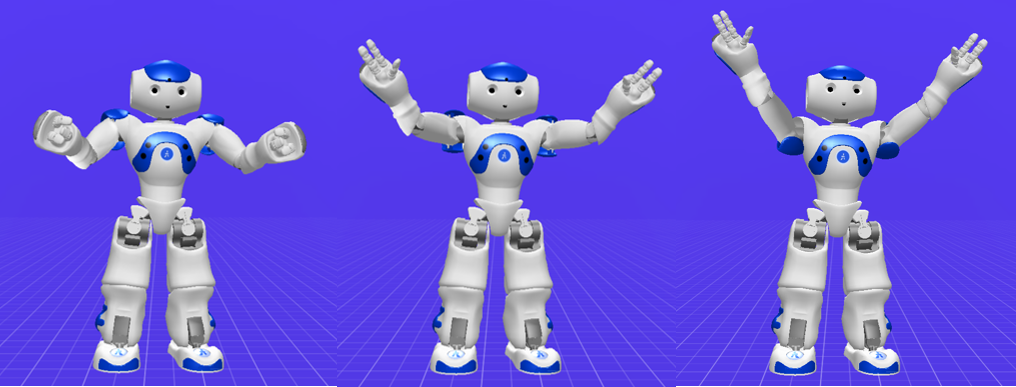
\includegraphics[width=1.0\linewidth]{./BothUpComparison}
\caption{Sample gesture ('Both Up') in the sad, neutral and happy conditions demonstrating the different in the Extent parameter across conditions.}
\label{fig:BothUpComparison}
\end{figure}


\subsection{Speech Generation}
Cereproc's CereVoice Engine Text-to-Speech SDK was used to create all speech for the robot. The CereVoice engine was selected because it supports a number of Speech Synthesis Markup Language (SSML) tags for voice modification which would allow application of the SIRE framework but also offers pre-defined emotional tags for generating emotional speech. The supported SSML tags identified for mapping onto SIRE parameters are listed in Table 3.3; however for this project it was decided, providing the testing and validation of the voice yielded good results, to use the pre-determined emotional tags. The main aim of this project was to investigate robot to human interpersonal emotion transfer (IET) and the impact of affective communication, rather than to design and evaluate the best emotional expression system. For this reason the simplicity and speed of implementation of the SSML tags made them the preferred choice. Future work would also be to see how well SIRE values could be extracted from this speech in the way that Lim et al. used actor samples with their system \cite{lim2011converting}. All speech files were generated in advance of the experiment and accessed as .wav files within the robot's control script. 

\begin{table}
\begin{center}
\begin{tabular}{|c|c|}
	\hline SIRE Parameter & Cerevoice Tag(s)\\ 
	\hline Speed & rate \\ 
	\hline Intensity & rate, duration \\ 
	\hline Regularity & break, duration \\ 
	\hline Extent & pitch range, pitch contour \\ 
	\hline 
\end{tabular}
\caption{Specific initial SIRE values used for initial testing.}
\end{center}
\end{table}

\subsection{Choregraphe}
Implementation of the SIRE algorithm and control of the NAO was undertaken within Softbank Robotics' graphical user interface, Choregraphe. Individual gestures with SIRE parameterisation were scripted in Python and embedded in a Choregraphe box which allowed for easy slider-manipulation of each SIRE value. All other aspects of control e.g. making the robot stand, turning LEDs on and off, reading touch sensors etc. were achieved using standard Choregraphe library boxes. 

\section{Testing \& Validation of Emotion Expression}
Three emotion recognition experiments were carried out in order to test the initial SIRE values described above. The first two tested emotion recognition in speech only and gesturing only, the third tested combined speech and gesturing. Testing each modality independently at first allowed for validation of the CereVoice emotional SSML tags and SIRE framework. Testing the combined performance allowed for validation of the final system as intended for use in the main HRI experiment. The speech and gestures used for testing were based on a draft of the main HRI experiment design. 

All three experiments were administered through an online survey in which participants were asked to watch and/or listen to a video and rate the emotional state of the robot or speaker (video screen was a simple title slide for the voice only condition). The same 16 participants were recruited for experiments one and two covering the voice only and gesturing only conditions; a new set of 25 participants were recruited for the combined condition. All surveys consisted of 4 samples of each condition, neutral, happy and sad, and the order of the videos was randomised for each participant. Percentage recognition results for each condition are given in Table 3.4; it can be seen that they are in line with Lim et al.'s reported result of 60\%+ . 

\begin{table}
\begin{center}
\begin{tabular}{|c|c|}
	\hline Condition & Recognition\\ 
	\hline Voice Only & 60.4\% \\ 
	\hline Gesturing Only & 68.2\% \\ 
	\hline Voice + Gesturing & 65.0\% \\ 
	\hline 
\end{tabular} 
\caption{Emotion recognition results across voice only, gesturing only and voice plus gesturing combined.}
\end{center}
\end{table}

Chi-square contingency table analyses were performed to check whether the intended emotion was identified significantly more frequently than the other options in each condition. This was always found to be the case with $\chi^{2}(1,300) = 8.85 - 54.6$ and $p < 0.01 - 0.05$. Contingency table analyses were also performed to check the variation in recognition and te number of extreme emotion (i.e. very happy or very sad) choices across the conditions. Overall recognition did not vary significantly but the number of extreme emotion choices significantly increased between the voice only and voice plus gesturing conditions $\chi^{2}(1,492) = 5.66, p <0.05$. This is discussed further in Section 5.1.1. Based on these results it was decided to leave the initial SIRE values unchanged and to use the CereVoice emotion tags for generating the robot's speech, rather than extending the SIRE framework to include voice manipulation. 

\section{Human Robot Interaction Experiment Design}
\subsection{Interaction Context}

An imitation based robot-led exercise session was chosen to provide a contextualised HRI activity for testing the impact of affective robot communication. An imitation based activity was preferred as it inherently encourages the participant to focus on the robot's behaviour; Xu et al. used a gesture imitation game for this reason \cite{xu2014robot}. However, there is psychological evidence that winning or losing at a game can influence mood, attitude and likelihood of further game participation \cite{ward1988promotional}. It was therefore decided that a game based interaction should not be used in order to avoid any unintended emotional impact on participants. 

The use of robot exercise instructors has been investigated in multiple HRI studies (e.g. \cite{fasola2010robot}, \cite{goetz2002cooperation}, \cite{gockley2006encouraging}). Specifically relevant to this project is Fasola and Mataric's work on a robotic arm exercise instructor for the elderly \cite{fasola2010robot} which essentially results in the same robot interaction as Xu et al.'s set-up \cite{xu2014robot} but contextualised as a workout rather than a game. It was therefore decided to design an arm gesture exercise session in line with Fasola and Mataric's work which used the gestures employed by Xu et al. in order to allow for maximum comparison between the results from those works and this project. 

Other work by Tapus and Mataric investigated the effect of robot personality on participant's motivation to do repetitive and monotonous stroke exercises \cite{tapus2008user}. Participants were asked to do as much of each exercise as they felt necessary and this number was recorded as a quantitative measure of motivation. Similar techniques have been employed in other HRI studies such as Nakagawa et al.'s investigation of robot touch and monotonous task motivation \cite{nakagawa2011effect} and Goetz and Kiesler's study of robot seriousness and exercise regime compliance \cite{goetz2002cooperation}. Based on this it was decided that the robot-led exercise session should consist of one mandatory gesture set (in order to provide an opportunity for emotion contagion to occur) followed by a series of voluntary rounds, the number of which completed by each participant being a quantitative measure of their motivation. An overview of the interaction flow can be seen in Figure \ref{fig:SimpleInteractionFlow}.

\begin{figure}
\centering
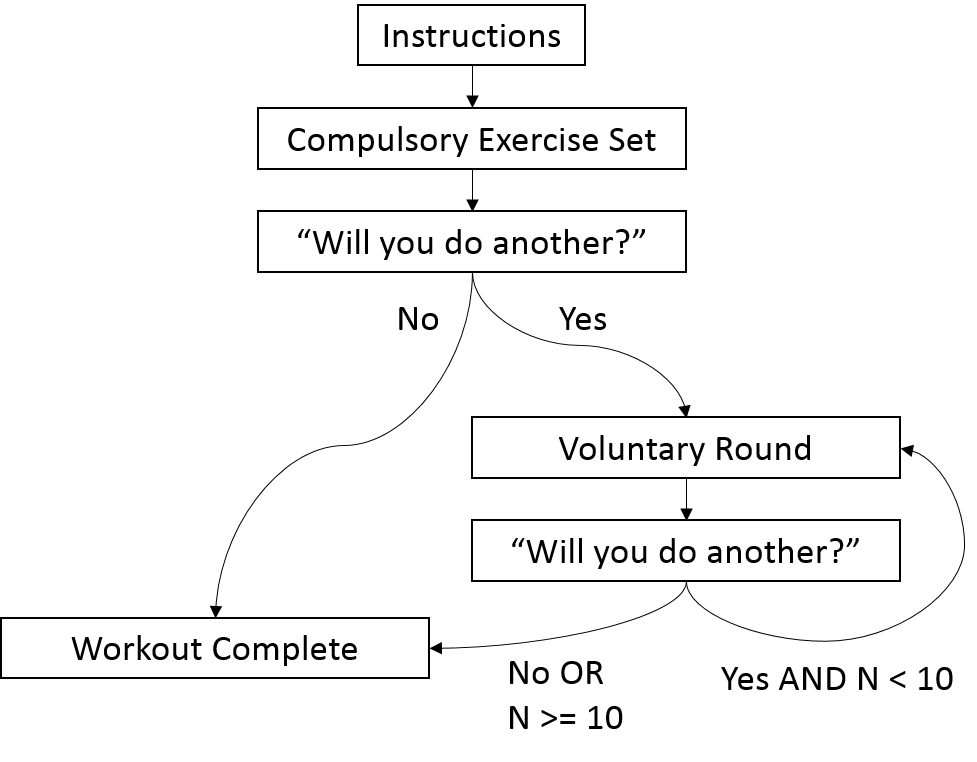
\includegraphics[width=0.7\linewidth]{./SimpleInteractionFlow}
\caption{Simplified interaction flow diagram showing the use of voluntary rounds up to a maximum N = 10.}
\label{fig:SimpleInteractionFlow}
\end{figure}

\subsection{Robot Script}

The NAO was programmed firstly to stand, read out the initial instructions and ask the participant to touch its head if they were ready to begin; at this point the eyes turned green to indicate it was waiting for a response. Once the robot sensed a head touch it proceeded to go through the mandatory round, after which it asked whether the participant would like to do another round and to touch the head for yes or foot for no. Again the eyes turned green in order to indicate a response was required. If the participant pressed the head, indicating they wished to continue, then the robot went through another round of exercise and repeated the question again. If the participant pressed the foot, indicating they wished to stop, then the robot thanked them for exercising with it and sat down. Physical touch rather than speech recognition was used for this continuation check in order to reduce the likelihood of incorrect classifications which would nullify the quantitative measure of voluntary exercise rounds. The number of voluntary rounds was capped at 10 using a for loop; when this number was reached the robot told the participant they had done the maximum amount of exercise for today and sat down as in the foot touch situation. 

Each round of exercise consisted of four gestures followed by a verbal confirmation that another round had been completed and a positive encouragement; this is depicted in Figure \ref{fig:ExerciseRound}. The gestures were taken directly from those used in Xu et al.'s imitation game \cite{xu2014robot} and are listed in Table 3.5, which also contains the list of encouragements used. For gestures involving the left and right the instructions were reversed to the physical action such that participants had to mirror the robot; for example when the robot said "put your right arm up" it actually raised its left arm, which participants mirrored by raising their right arm. The mandatory round of exercise was the same for all participants; each voluntary round was chosen randomly in real time from ten alternative, pre-determined options using a random number generator. The gesture and encouragement combinations used in each of the ten options were also generated randomly prior to scripting the robot's control programme. The robot did not monitor the participants' performance in any way. 

\begin{figure}
\centering
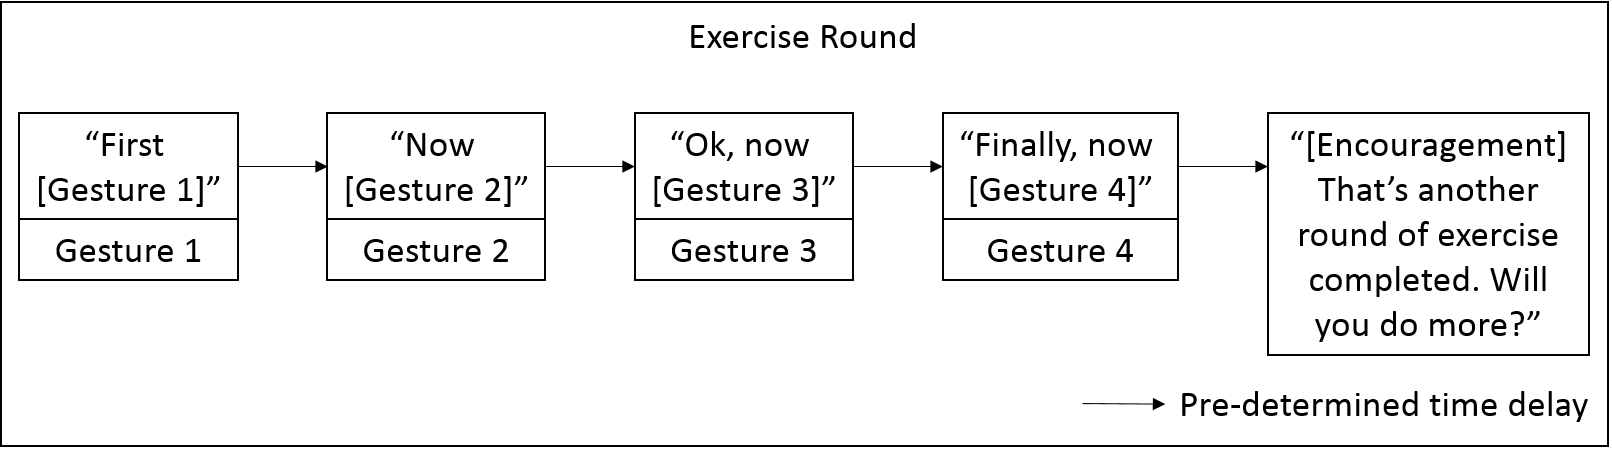
\includegraphics[width=1\linewidth]{./ExerciseRound}
\caption{Overview of each exercise round which consisted of four gestures and an encouraging acknowledgement that another round had been completed. The robot did not monitor the participant in any way; a pre-determined time delay was used to space out gestures.}
\label{fig:ExerciseRound}
\end{figure}

\begin{table}
\begin{center}
\begin{tabular}{|l|p{7cm}|}
\hline Gesture Instructions & put your right arm up \newline put your right arm down \newline put your left arm up \newline put your left arm down \newline put both arms up \newline put both arms down \newline put your right arm up and left arm down \newline put your left arm up and right arm down \\ 
\hline Encouragement & great, well done \newline awesome \newline you're doing really well \newline fantastic \newline excellent \newline nice \newline good job \\ 
\hline 
\end{tabular}
\caption{The full set of gestures and encouragement from which exercise rounds were generated.} 
\end{center}
\end{table}

\subsection{Hypotheses \& Measures}
The four main hypotheses investigated in this project are as follows:

\begin{itemize}
	\item[H1] Participants in the valenced conditions will demonstrate an emotional state of matching valence after interacting with the robot, (i.e. emotion contagion will occur)
	\item[H2] Participants will recognise the intended emotional state of the robot when interacting with it
	\item[H3] Emotion expression will have an impact on human motivation and enjoyment 
	\item[H4] Emotion expression will have an impact on perception of the robot
\end{itemize}

H1 describes the expectation that some evidence for robot to human emotion contagion will be found. This is based on the fact that Xu et al. found some evidence for contagion during their robot-led gesture imitation game on which this project draws heavily \cite{xu2014robot}. H2 states that participants will be able to recognise whether they are working with the sad, happy or neutral robot and is based on the results of the pre-test work described in Section 3.2 as well as Xu et al.'s and Lim's positive emotion recognition results \cite{xu2014robot} \cite{lim2011converting}. 

H3 and H4 describe the expectation that the use of affective movement and speech in the exercises session context will have an impact on people's behaviour, enjoyment and perception of the robot. This is based firstly on the human psychology literature discussed in Section 2.1.1, e.g. the observation that people may take different amounts of drink from a jug depending on whether it is offered by a smiling face or frowning face. In addition, it is expected based on HRI studies which have demonstrated how changing a robot's behaviour can change participant behaviour and perception; for example Nakagawa et al.'s study of active touch and motivation \cite{nakagawa2011effect} or Chidambaram et al.'s study of communication cues and persuasion \cite{chidambaram2012designing}. Overall these hypotheses can be grouped under two key features of interest; robot to human emotion contagion and the impact of affective communication on HRI. The experimental measures relevant to each area of interest and the specific hypotheses they relate to are listed in Table 3.6.  

\begin{table}
\begin{center}
\begin{tabular}{|l|p{7cm}|p{3.8cm}|}
\hline Feature of Interest & Related Measures & Relevant Hypotheses \\ 
\hline Emotion Contagion & Word completion task \newline Emotional state (of robot and self) & H1 \newline H1 \& H2 \\ 
\hline Impact on HRI & Number of exercise rounds voluntarily completed \newline Enjoyment Likert scale \newline Reason for stopping Likert scale \newline Perceived usefulness Likert scale \newline Selected Godspeed Questions \newline Open feedback/comments &  H3 \newline \newline H3 \newline H3 \newline H4 \newline H4 \newline H4 \\
\hline 
\end{tabular} 
\caption{Key features of interest in the exercise session experiment with related measures and relevant hypotheses.} 
\end{center}
\end{table}

Table 3.6 shows two measures for H1; a word completion task and a direct emotional state assesmment question. These represent implicit and explicit measures respectively. As discussed in Section 2, some emotion contagion effects in humans may be subconscious and so it was deemed important to also include an implicit mood measure in the surveying of participants. Measuring mood with both explicit and implicit measures also allows for a comparison between participants' conscious and subconscious feelings. Video coding analysis to look for visual emotional cues such as smiles and laughter was considered as an implicit measure, however this was deemed impractical for this project for two reasons. Firstly, video coding is a timely procedure which requires individual analysis of each participant; this is particularly an issue given the large number of participants involved in this study. Secondly, it has been demonstrated that cues of being watched can increase compliance in people undertaking something voluntary \cite{bateson2006cues}. Therefore it was hypothesised that the use of video recording equipment and participants' knowledge that they were being filmed may affect the number of voluntary exercise rounds they chose to complete. Based on this a participant task based approach was preferred; a word completion test was chosen for this purpose and is discussed in more detail below. 

Quantitatively measuring participant motivation was one of the key aims of this project. As discussed in Section 3.3.1 the use of voluntary exercise rounds as a quantitative measure is inspired by previous studies which have used voluntary participation as a quantitative measure (e.g. \cite{gockley2006encouraging}, \cite{nakagawa2011effect}). A number of Likert style questions were derived in order to evaluate differences in participants' experience and perception of the robot across the different emotional conditions. Firstly participants were asked how much they enjoyed working out the robot. Secondly, based on questions asked by Gockley and Mataric, participants were asked whether they stopped more due to boredom or tiredness and how useful the robot was in getting them to exercise \cite{gockley2006encouraging}. A number of relevant questions taken from The Godspeed Questionnaire Series, a standardised set of HRI questionnaires \cite{bartneck2009measurement} were also included in the survey. Finally participants were asked to leave any additional thoughts, comments or feedback in an open text box question. A blank version of the survey can be seen in Appendix B.


\subsubsection{Word Completion Test}

Word completion tests require the participant to complete a word stem, a word with one or more missing letters, which has multiple possible completions. In HRI studies, such tests have typically been used measure death thought accessibility linked to the Uncanny Valley effect \cite{koschate2016overcoming}; but they have also been used in human psychology studies in order to measure emotional state \cite{dewall2007terror}. Other implicit mood measures considered include a memory recall test \cite{seibert1991irrelevant} or creative task performance \cite{isen1987positive}. Creative task performance was disregarded because it tests only for positive mood, meaning an alternative test would have been required for participants in the negative condition. In the work on mood and memory recall emotional states were induced in participants using strongly valenced statements and in their discussion of the measured impact on memory recall the authors state memory might be affected due to an increase in irrelevant thoughts linked to these statements \cite{seibert1991irrelevant}. It is not clear how well the memory measure would therefore work on more subtle emotional manipulation.

A word stem list was generated using Bradley and Lang's Affective Norms for English Words (ANEW): Instruction Manual and Affective Ratings \cite{bradley1999affective}. Firstly all words with a valence greater than seven (positive), less than three (negative) and exactly five (neutral) were identified. Possible word stems and alternative completions were then considered for each of the valenced words to find word stems which had one valenced completion (positive or negative only) and one or more neutral completions. For the neutral words word stems with only neutral completions were selected. Finally the word frequencies of these alternative completions were compared and all word stems with a difference greater than one in any possible completion were discarded. Eleven neutral, six positive and six negative words were selected from the remaining pool to generate an initial word list for the completion activity. 

A pretest was then carried out to examine completion frequencies of the valenced words in a relatively neutral context (N = 8). Valenced word stems which were completed by more than 50\% of participants were discarded and replaced with others from the pool described above. The final word stems and possible completions are given in Appendix A. All participants completed the entire word list of negative, positive and neutral word stems. This is shown in question 1 of the participant survey presented in Appendix B. Whilst outside the scope of this project, further work would be to undertake full validation of the word stem list using controlled emotion induction such that it might be used as a standardised implicit measure of emotional state. 

\subsection{Experimental Procedure}
A total of 62 participants (18 male and 44 female) aged between 21 and 60 (Mean = 31.7 SD = 8.72) were recruited for the experiment and randomly assigned to one of the three conditions resulting in 21 subjects in the happy and neutral conditions and 20 subjects in the sad condition. The quantitative data for one subject in the happy condition was discarded due to a fire alarm disrupting the experiment. Participants were offered a $�5$ Amazon voucher as compensation for taking part in the experiment. 

Participants were first asked to read through an experiment information sheet which stated that the NAO was programmed to guide them through an arm exercise session typically used by older adults and the disabled to keep fit. It was explained that each round of exercise consisted of 4 gestures and that the first round of exercise was mandatory, after that NAO would ask the participant if they wanted to continue or stop and that they could stop exercising whenever they wanted to; this was highlighted in bold text. 

A demo was then given to show the participants what to expect and how to safely interact with the robot in terms of touching the head or foot to indicate they wanted to continue or end the exercise session. At this point it was verbally pointed out again to the participants that all exercise rounds after the first were voluntary and they could stop at any time. The experimenter then launched the main experiment script and left the room once the robot was seen to be working correctly, returning when the exercise session was complete. The experimental set-up can be seen in Figure \ref{fig:ExpImage}. 

Once the exercise session was complete participants were asked to complete an online survey containing the word completion task, perception of the robot questions and robot/self emotional state questions described in Section 3.3.3. Participants were then asked to read a debrief sheet which explained the underlying study of affective communication and its impact on HRI with a note not to discuss this with any other potential participants until after they had also completed the experiment. Finally participants were given a final chance to ask any questions about or discuss the research further with a note made of any additional qualitative feedback. 

\begin{figure}
\centering
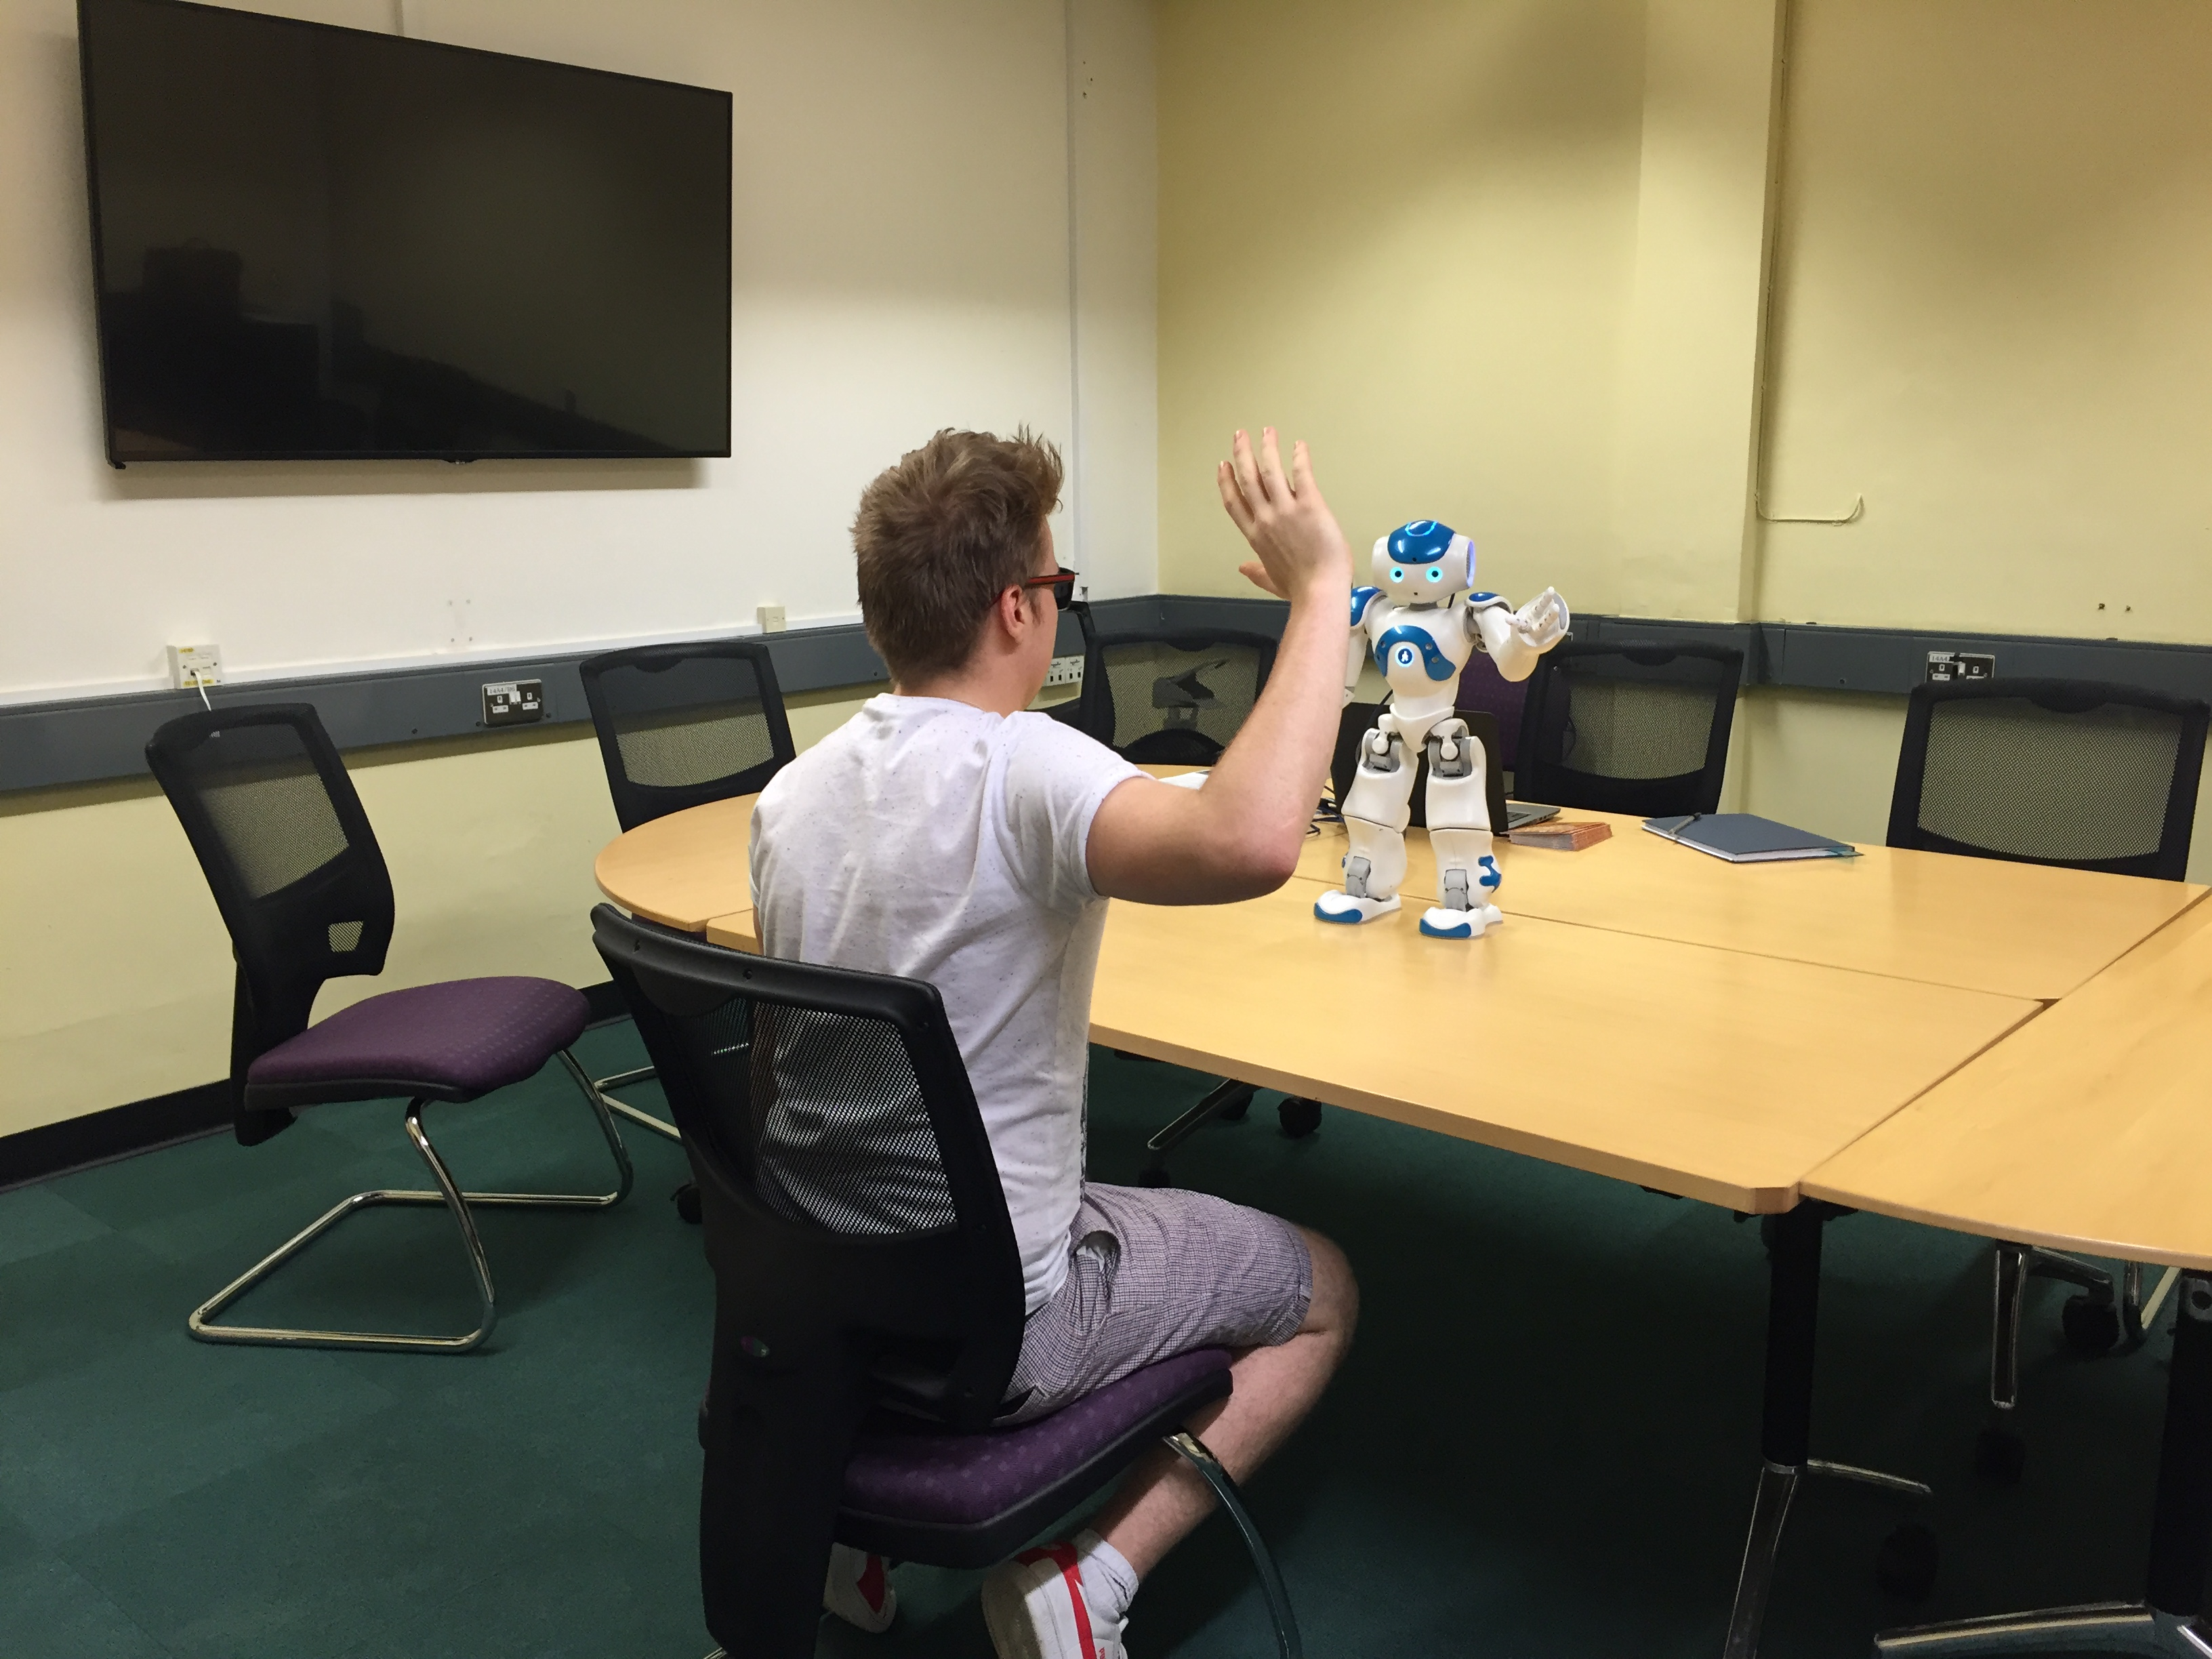
\includegraphics[width=0.7\linewidth]{IMG_5290}
\caption{A participant interacting with the robot during the NAO-led exercise session experiment.}
\label{fig:ExpImage}
\end{figure}

\chapter{Results}

\section{Robot to Human Emotion Contagion}
\subsection{Robot Emotion Recognition}
Figure \ref{fig:RobotMood} shows participants' perception of the robot's emotional state across conditions; essentially representing a manipulation check of whether the intended emotions were recognised. Clearly this was not the case. Almost all participants judged the robot to be either neutral or happy with roughly an equal split between the two. Interestingly the largest difference was in the happy condition, where the robot was judged to be neutral more often than happy, however a chi-square contingency table analysis showed this wasn't significant.  

\begin{figure}
	\centering
	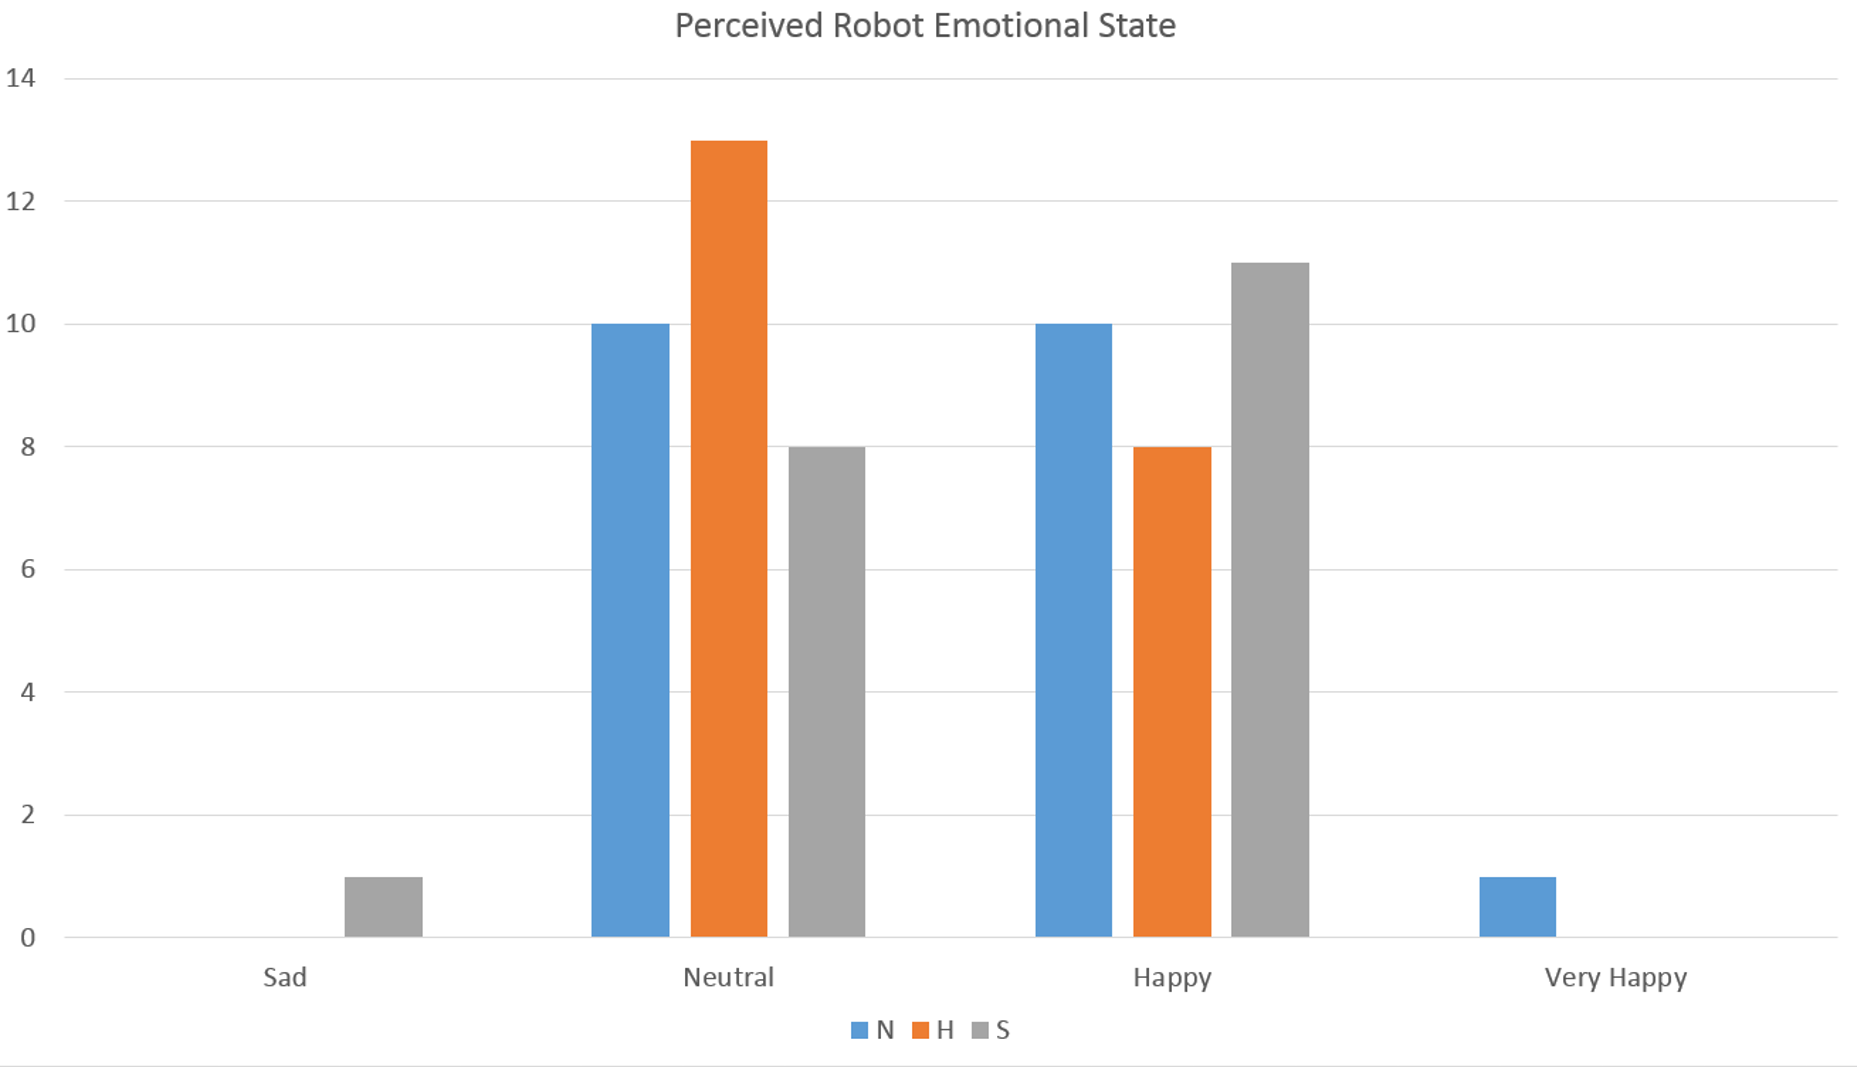
\includegraphics[width=\linewidth]{RobotMood}
	\caption{Robot emotional state as perceived by participants from each emotional condition; essentially representing a manipulation check for emotion recognition.}
	\label{fig:RobotMood}
\end{figure}

\subsection{Human Mood Measures and Manipulation Check}
The mean number of positive, negative and total emotive word completions per participant are listed in Table 4.1. One way ANOVA tests with the number of each were carried out in order to check for differences across the three emotion conditions. It can be seen in Table 4.1 that the average number of emotive completions did increase between the neutral and emotive conditions; however the ANOVA analysis yielded no significant difference. Figure \ref{fig:SelfAssessedMood} shows the number of participants that selected each of the possible emotional state descriptor faces to describe their own emotional state when interacting with the robot; the similarity in response across conditions is clear and therefore no additional statistical analysis was undertaken. In all conditions the majority of participants indicated they were happy and no participants indicated they were sad or very sad whilst interacting with the robot. 

\begin{table}
\begin{center}
\begin{tabular}{|c|c|c|c|}
	\hline & M(Positive) & M(Negative) & M(Total) \\ 
	\hline Neutral & 1.19 & 1.05 & 2.24\\ 
	\hline Happy & 1.62 & 1.05 & 2.67 \\ 
	\hline Sad & 1.43 & 1.24 & 2.67 \\ 
	\hline 
\end{tabular} 
\caption{The average number of emotive word stem completions by participants in each emotional condition.} 
\end{center}
\end{table}

\begin{figure}
\centering
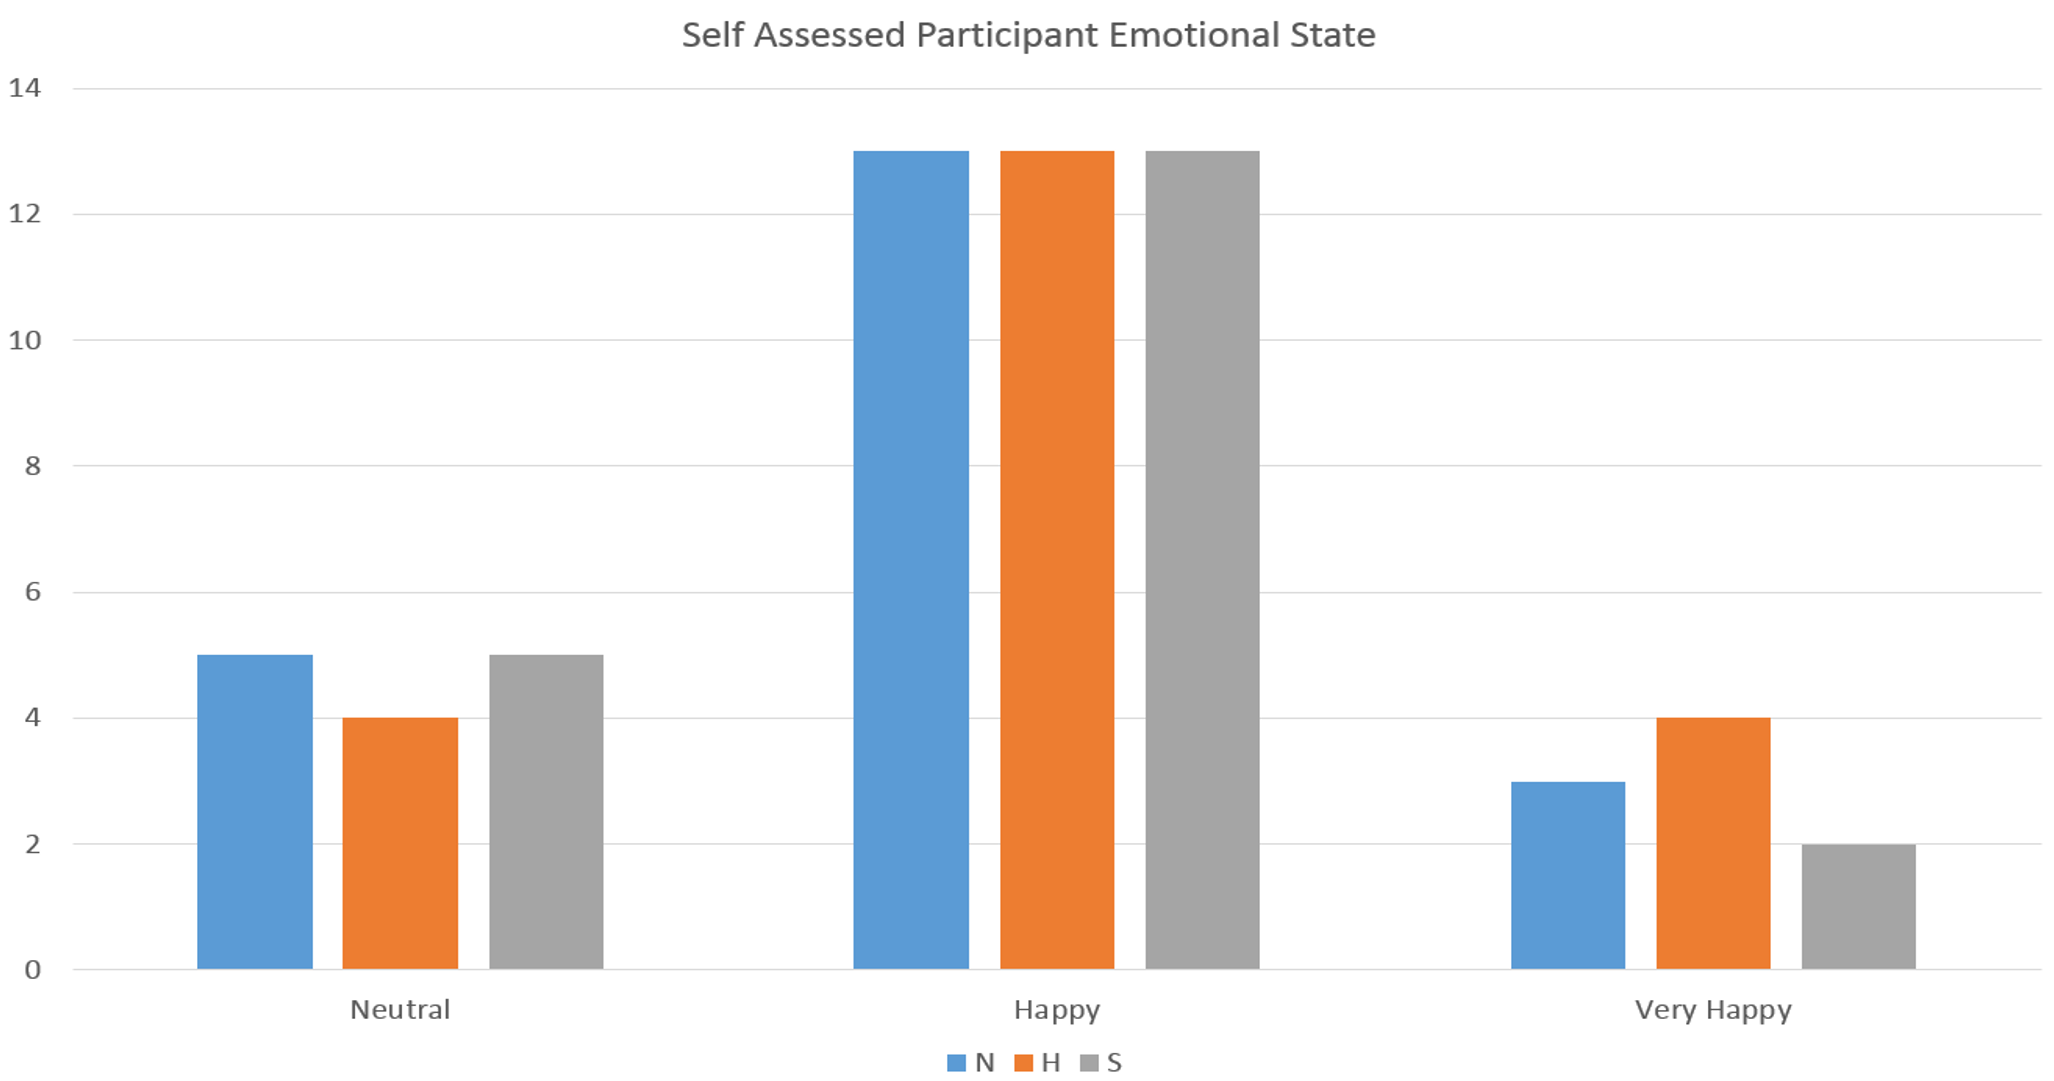
\includegraphics[width=\linewidth]{SelfAssessedMood}
\caption{Self assessed emotional state as perceived by participants from each emotional condition.}
\label{fig:SelfAssessedMood}
\end{figure}

\section{Impact of Affective Communication on HRI}
\subsection{Voluntary Exercise Rounds \& Closed Survey Questions}
The mean number of voluntary rounds undertaken by participants in each condition is listed in Table 4.2. This data suggests that people exercised less with the happy robot however a one way ANOVA analysis yielded no significant difference between conditions $(p = 0.14)$. 

\begin{table}
\begin{center}
\begin{tabular}{|c|c|}
	\hline & Average Rounds\\ 
	\hline Neutral & 8.67 \\ 
	\hline Happy & 7.33 \\ 
	\hline Sad & 8.15 \\ 
	\hline 
\end{tabular} 
\caption{The average number of voluntary exercise rounds undertaken by participants from each emotional condition. } 
\end{center}
\end{table}

One way ANOVA analyses were also carried out for each of the Likert and semantic difference scale survey questions; no significant differences were found in the responses to any question across the three emotion conditions. 

\subsection{Open Question and Additional Qualitative Data}
Comparing comments across the three emotional conditions further suggested a lack of affect-related impact with the same themes appearing in all three. For example, at least one participant in all three conditions commented that the robot was not emotional or that they found it hard to answer the survey questions covering emotional state and 'human, emotional items'. Another consistent theme was the lack of responsiveness or interactiveness reducing the possibility of rapport and the liveliness/lifelikeness of the robot. Positive and negative feedback was spread relatively evenly across conditions with contradictions present in each condition. For example, whilst lack of responsiveness was a consistent theme, some participants stated the robot was fun and interactive. Additionally the robot's voice was described both as friendly and encouraging but also cold and harsh.

Further feedback was gathered informally from participants once they had read the debrief sheet and were invited to ask any questions or discuss the emotional aspect of the work in more detail. Many in the emotionally valenced conditions were surprised to find out that the robot was supposed to look sad or happy, but recognised the difference when then shown the oppositely valenced or neutral condition. Some participants in the sad condition noted that they wouldn't have guessed the robot was sad because of the positive verbal encouragement it gave between rounds. Interesting feedback specific to the exercise session context of the experiment included comments about motivation coming from fear of judgement by another person which couldn't be achieved with a robot.

\chapter{Discussion}

This chapter presents a discussion of the results documented in Chapter 4. Emotion recognition was high in the validation experiments but was not achieved in the exercise session. This is likely due to the between-subject experiment design; previous work and the validation experiments undertaken in this project utilised within-subject testing. Additional analysis of the validation results yielded the interesting observation that the use of gestures seems to increase the perceived extremity of the robots emotional state. Results from the exercise session experiment suggest that the addition of affective communication had very little impact on participants; however this is likely due to the lack of emotion recognition described previously. 

\section{Emotion Recognition in Robot Gesture and Voice}

\subsection{Gestures and Perceived Emotion Extremity}
Although an aside from the main project investigation, the finding that combining voice and gesturing significantly increased the perceived extremity of emotion compared to voice only is noteworthy. Psychology studies have shown that gesturing is an integral part of human-human interaction \cite{kendon2004gesture} \cite{mcneill1992hand} and whilst research in the area of robot gesturing has generally shown its utility \cite{bremner2009conversational} \cite{bremner2015efficiency} there has been some doubt over gesture-speech integration in robot compared to human communicators \cite{bremner2015}. The results found in this work however suggest that even non-semantic gestures can amplify implicit vocal effects and are therefore worth implementing on a robot designed to portray emotion.

\subsection{Recognition in Pretesting vs Exercise Session}

One of the most interesting results found in this project is the contrast in emotion recognition between the gesture and voice pretesting and the final exercise session experiment. Participants undertaking the pretest reliably recognised the intended emotion successfully whereas participants undertaking the exercise session failed to do so. One possible reason for this is experiment context and set-up; in the pretesting participants were shown each of the emotional conditions multiple times and were asked each time to judge the robot's emotional state, whereas in the exercise condition participants only experienced a single emotional state and were only asked once, at the very end of the experiment, to judge that emotional state. Participants completing the exercise session were also under the impression that they were evaluating the use of NAO as an exercise instructor, whereas it is likely participants in the gesture and voice pretesting realised the goal of the pretest and the overall aim of the work to make NAO look emotional and may have therefore been subject to a demand effect. This is in line with qualitative feedback from the exercise session experiment with some participants saying they thought that robots couldn't be emotional and therefore they never would have considered the robot may have an emotional state. 

Successful emotion recognition in the SIRE and voice pretesting was expected based on results from Lim et al.'s SIRE emotional gesture work \cite{lim2011converting} and Masuda and Koto's LMA emotional gesture work \cite{masuda2010motion}. Masudo and Koto used a similar testing method to the pretesting utilised in this project. Participants were shown a total of eight sample behaviour pairs, each one consisting of a `basic' (non-emotional) gesture followed by the same gesture adjusted to demonstrate a target emotion. There were three basic gestures and eight emotional versions of each of those covering the four emotions of pleasure, anger, sadness and relaxation at the two strengths of weak and strong. Order and choice of each emotional gesture was randomised and after each individual gesture participants were asked to estimate the robot's emotions. 

Lim et al.'s emotion recognition experiments were also set up in a similar way. In their voice only experiment participants were asked to watch a virtual NAO perform an arm extension gesture and then given five seconds to choose the emotional state of the robot from happy, sad, angry or scared. This was repeated sixteen times with four samples of each emotion presented in a random order. In their voice and motion experiment the arm gesture used each time was chosen at random, however participants were still subject to four samples of each of the four different target emotions. In summary, as with the pretesting done in this work, previous experiments were of a within-subject design whereby participants saw different emotion conditions and could therefore see a relative difference between gestures. In addition participants in the above experiments were probably aware of the aim of the work (to design emotional robots) which may have caused a demand effect as discussed previously.

Successful emotion recognition in the exercise session experiment was expected primarily based on the results of Xu et al. who found that participants were able to distinguish between negative and positive mood in their NAO gesture imitation game experiment \cite{xu2014robot}. Participants played the imitation game twice with the robot, once in each emotional condition and then, after the second game, were asked to score the robot's valence and arousal. Therefore, as with the pretesting work of this project, Lim et al's experiments \cite{lim2011converting} and Masuda and Koto's experiment \cite{masuda2010motion} as described above, participants witnessed multiple emotion conditions before being asked to describe the robot's emotional state. In summary, all previous emotion recognition work cited in the literature has utilised within-subject experiment design. This is in direct contrast with the between-subject exercise session experiment undertaken for this project in which participants worked with the robot in one of the emotional conditions only; meaning this work is the first to test robot emotion recognition when participants witness a single condition only. Tsai et al.'s virtual agent study was also between-subjects and they found strong evidence for emotion recognition and contagion; however their agent's utilised facial expression for emotion recognition \cite{tsai2012study}. Based on this it could be that emotion recognition from voice and gesture alone with no facial expression may only be possible in relative terms, i.e. it is possible to identify the robots emotional state only after experiencing alternative conditions and not when interacting with the robot for the first time. 

This has interesting implications for the perception of robots based on prior knowledge and/or expectations. It may be that when people are listening to other humans, emotion in neutral speech or speech in a different language can be detected because it is known that humans can and do express emotion in this way. Similarly in the within subject previous work and pretesting that explicitly asked participants for the emotional state of the robot, thereby implying it had an emotional state at all, people were possibly aware that the robot could display emotions and therefore were able to spot them. Further investigation is required to test this hypothesis.

Another possible reason for the lack of emotion recognition in this work compared to Xu et al.'s is the choice of questioning method used to test robot emotion perception. Xu et al. asked participants to numerically rate the robot's valence and arousal whereas this work utilised discrete pictorial smiley-face/emoji style descriptors (these can be seen in Appendix B). As discussed in Section 4.2.2; a consistent theme in participants feedback was that they found it difficult to answer emotion questions about the robot because robots don't or can't have emotions. The use of valence and arousal rather than discrete, human based emotions may not have had this same effect on participants and so such measures might be more likely to get positive results. Finally, the use of encouragement phrases in the exercise session experiment may have prevented or reduced emotion recognition, particularly in the sad condition. Xu et al. did not use such phrases; their robot only told participants whether they were correct or incorrect. Previous work both in human psychology \cite{neumann2000mood} \cite{scherer2000cross}) and human robot interaction (HRI) \cite{lim2011converting} suggests that emotion can be portrayed through any speech. However it may be that in affective robot communication which is limited to voice and gesture only, whilst the portrayed emotion may be recognisable in neutral speech, it may be too subtle to overcome the emotion associated with emotive exclamations. For example the slow movements and deep voice of the sad condition were not enough to overcome the positive exclamations given at the end of each exercise round. This would align with feedback from participants in the sad condition as discussed in Section 4.2.2. 

\section{Robot to Human Emotion Contagion}
The results of Xu et al. \cite{xu2014robot} who found evidence for contagion in a NAO led gesture imitation game, the good emotion recognition results found in pretesting of this work and the fact that Tsai et al. found evidence for emotion contagion in a between-subject virtual agent experiment \cite{tsai2012study} would suggest that emotion contagion should have occurred during the NAO exercise session; however no evidence was found to support this. One possible reason for this is the lack of emotion recognition achieved in the exercise sessions; it could be that some level of concious emotion recognition is required in order for contagion to occur. Xu et al. and Tsai et al. both achieved emotion recognition as well as finding evidence for contagion, which would support this hypothesis. If this is the case and emotion recognition is required for contagion to occur then robot facial expression capabilities are likely to be crucial in scenarios where contagion is desired but users will not have multiple interactions with the robot. 

Other possible reasons for the lack of contagion include robot responsiveness and interaction context. In Xu et al.'s imitation game, the robot told the participant whether they were right or wrong after each gesture sequence \cite{xu2014robot}. This work did not utilise any personalised feedback between the robot and participant; as discussed in Section 4.2.2 this was noted by participants and highlighted as a reason the robot seemed less alive and less interactive, which may have had an impact on the potential for emotion contagion. Tsai et al. found that emotion contagion dropped off in situations where the virtual agent was presented in a contextual interaction and disappeared altogether in situations where participants had to make a strategic decision involving the agent \cite{tsai2012study}. Based on this it could be that the exercise session context and the cognitive loading of imitating the robot may have prevented emotion contagion, however this seems unlikely as the experiment was contextually similar to Xu et al.'s in which some evidence for contagion was found. 

\section{Impact of Affective Communication on HRI}
Previous HRI studies have shown that changes in robot behaviour can have an impact on human behaviour and perception of the robot. Particularly relevant to this project it has been shown that changes in the proximity and apparent 'engagement' of a mobile robot can have an impact on physical therapy compliance \cite{gockley2006encouraging} and that people comply more with an exercise regime presented by a serious robot than a happy robot \cite{goetz2002cooperation}. In terms of robot perception, Chidambaram et al. showed that the use of different robot communication cues can have an impact on perceived robot intelligence \cite{chidambaram2012designing} and Koschate et al. demonstrated that displays of emotion can reduce the uncanniness of humanlike robots \cite{koschate2016overcoming}. Therefore it was expected that in the exercise session experiment some differences would be seen in the number of voluntary rounds of exercise participants completed and the various robot perception measures across the different emotional conditions; however this was not the case. 

As discussed in the Section 5.1; participants failed to recognise the NAO's intended emotional state and no evidence was found for robot to participant emotion contagion. Therefore conclusions about the impact of affective or emotional communication can not really be drawn from the experiment results; instead it can only be said that changing the SIRE values of each gesture and the robot voice as described in Section 3.1 had little to no impact on participants' behaviour and perception of the robot. These changes are relatively subtle compared to those in the HRI studies cited above; for example the difference between Goetz and Kiesler's happy and serious robot was its actual audio script (fun and joking versus stating health related concerns). Gockley and Mataric and Chidambaram et al. both utilised changes in proximity, which in human-human interactions is known to have a large impact on compliance with a speaker \cite{buller1986effects}. As such the question of whether affective communication can have an impact on HRI still remains; it may be that if emotion recognition was achieved then the results from the exercise session experiment would have been different. This warrants further investigation and is discussed further in Section 6.2. 

\chapter{Conclusions}
The overall aim of this project was to investigate whether robot to human interpersonal emotion transfer (IET) can occur and, regardless of the result, what impact affective robot communication can have on human behaviour and perception of the robot in a real world context. The lack of emotion recognition achieved in the exercise session experiments means that these questions cannot be answered fully by this work; however a number of important conclusions and potential hypotheses for future work can be drawn. 

A specific objective of this project was to implement a method for generating functional/semantic free emotional expression on the NAO. This was achieved using a parameterisation model for gesturing and a commercially available text to speech generator for voice. Emotion recognition was achieved in within-subject validation experiments but not in the between subject exercise session experiments. Another objective was to conduct a contextualised human robot interaction (HRI) experiment with appropriate measures for investigating the effects of affective communication. Inspiration for experimental measures was taken from a range of HRI and psychology studies and a specialised word completion task was designed in order to implicitly test emotional state. However, the lack of emotion recognition in the final exercise session experiments means that the impact of affective robot communication was not tested as originally intended. 

Recommendations for re-addressing the impact of affective communication are given in Section 6.2; however a number of conclusions can still be drawn from the presented work. Firstly, the results of the exercise session experiment suggest that robot to human IET can not occur if concious emotion recognition does not occur. In addition, comparing the results of this work to published literature suggests emotion recognition with robots using voice and gesture only can only occur if users witness the robot in different emotional states; however this may not be the case for robots with facial expression capabilities or where participants are expecting or aware of the robot's emotion expression capabilities. Finally, in a slight aside, results from the emotion expression validation suggest that gesturing can increase the perceived extremity of a robot's emotional state.

Of most importance to real world robotics applications is the lack of emotion recognition in the exercise session experiments. This suggests that voice and gesture alone are unlikely to be sufficient for achieving emotion recognition in single or infrequent interactions, therefore reducing the potential for IET and its associated benefits. Demonstrated example situations where this may be an issue include a robotic doctor's receptionist or store assistant; both of which Softbank Robotics' Pepper robot has been used for \cite{pepperNews} \cite{pepperNews2}. Also of note for real world applications is that it is worthwhile to implement gesturing on a robot which is designed to portray emotion as this can increase the perceived emotion extremity. 

\section{Limitations of this Work}

As discussed previously the lack of emotion recognition in the final exercise session experiment means that this project has not investigated the impact of affective robot communication as originally intended. This is the greatest limitation of the work carried out. More generally, whilst the exercise session context provided the real world applicability required by the project objectives, it also limits the applicability of the some of the qualitative feedback provided by participants. 

\section{Recommendations for Further Work}

An obvious piece of further work resulting from this project would be to re-run the exercise session experiment with some modifications such that emotion recognition is achieved. This would address the original aim of the project to investigate robot to human IET and the impact of affective robot communication. Based on the discussion presented in Section 5.1.2 this could be done in one of two ways. Firstly, the participants could witness the robot in multiple conditions during the experiment; for example the robot might be in the neutral state for giving an initial demonstration but then switch to the valenced condition for the actual arm exercise session. Alternatively some context could be given in order to explain the robot's emotional state, for example the robot could discuss a valenced event with the participants before undertaking the experiment. This must be carefully thought out however in order to avoid description of the valenced event itself having an impact on participants' emotional state.  

More generally there are two ways in which the investigation presented here could be extended. The first would be to undertake a long term interaction experiment whereby the robot has continued, regular interactions with participants. This could be in the style of Kidd and Breazeal's long term robot weight loss coach experiment \cite{kidd2008robots}, with a view to investigating the longevity of any impact caused by affective robot communication. The second would be to utilise facial expression for conveying emotional state and exploring the relative importance of facial expression compared to voice and/or gesture in emotion recognition and its consequences. 

\bibliographystyle{unsrt}
\bibliography{MyReading}

\appendix
\chapter{Word Stem List}

\begin{table}
	\begin{center}
		\begin{tabular}{|c|c|}
			\hline Word Stem & Completion(s) (All Neutral Only) \\ 
			\hline \_ O I S T & MOIST, HOIST \\ 
			\hline H U \_ L K & HUSK, HULK \\ 
			\hline K N \_ C K & KNICK, KNACK \\ 
			\hline \_ A T C H & BATCH, CATCH, HATCH, MATCH, PATCH \\ 
			\hline P A C \_ & PACE, PACT \\ 
			\hline \_ O R K & CORK, PORK, FORK, WORK \\ 
			\hline \_ E T A I L & RETAIL, DETAIL \\ 
			\hline R \_ G & RUG \\ 
			\hline S \_ I C K & SLICK, STICK \\ 
			\hline P I L \_ & PILE, PILL \\ 
			\hline V E \_ T & VENT, VEST \\ 
			\hline 
		\end{tabular} 
		\caption{Neutral completion only filler word stems for the word completion task} 
	\end{center}
\end{table}

\begin{table}
	\begin{center}
		\begin{tabular}{|c|c|c|}
			\hline Word Stem & Valenced Completion & Neutral Completion(s) \\ 
			\hline \_ I L L E R & KILLER & FILLER \\ 
			\hline \_ R I M & GRIM & TRIM, PRIM, BRIM \\ 
			\hline S H \_ N & SHUN & SHIN \\ 
			\hline W A \_ P & WASP & WARP \\ 
			\hline C R E E \_ & CREEP & CREED \\ 
			\hline \_ A S T Y & NASTY & TASTY \\ 
			\hline 
		\end{tabular} 
		\caption{Word stems derived from negatively valenced words with their original negative and alternate neutral completions.} 
	\end{center}
\end{table}
			
\begin{table}
	\begin{center}
			\begin{tabular}{|c|c|c|}
				\hline Word Stem & Valenced Completion & Neutral Completion(s) \\ 
				\hline J O \_ & JOY & JOG, JOT \\ 
				\hline D \_ N \_ E & DANCE & DENSE \\ 
				\hline \_ I F T & GIFT & LIFT, RIFT \\ 
				\hline B I \_ D & BIRD & BIND \\ 
				\hline B R A \_ E & BRAVE & BRACE, BRAKE \\ 
				\hline \_ A I R & FAIR & PAIR, LAIR, HAIR \\ 
				\hline 
			\end{tabular} 
		\caption{Word stems derived from positively valenced words with their original negative and	alternate neutral completions.} 
	\end{center}
\end{table}
						
\chapter{Exercise with NAO Survey}
\newpage
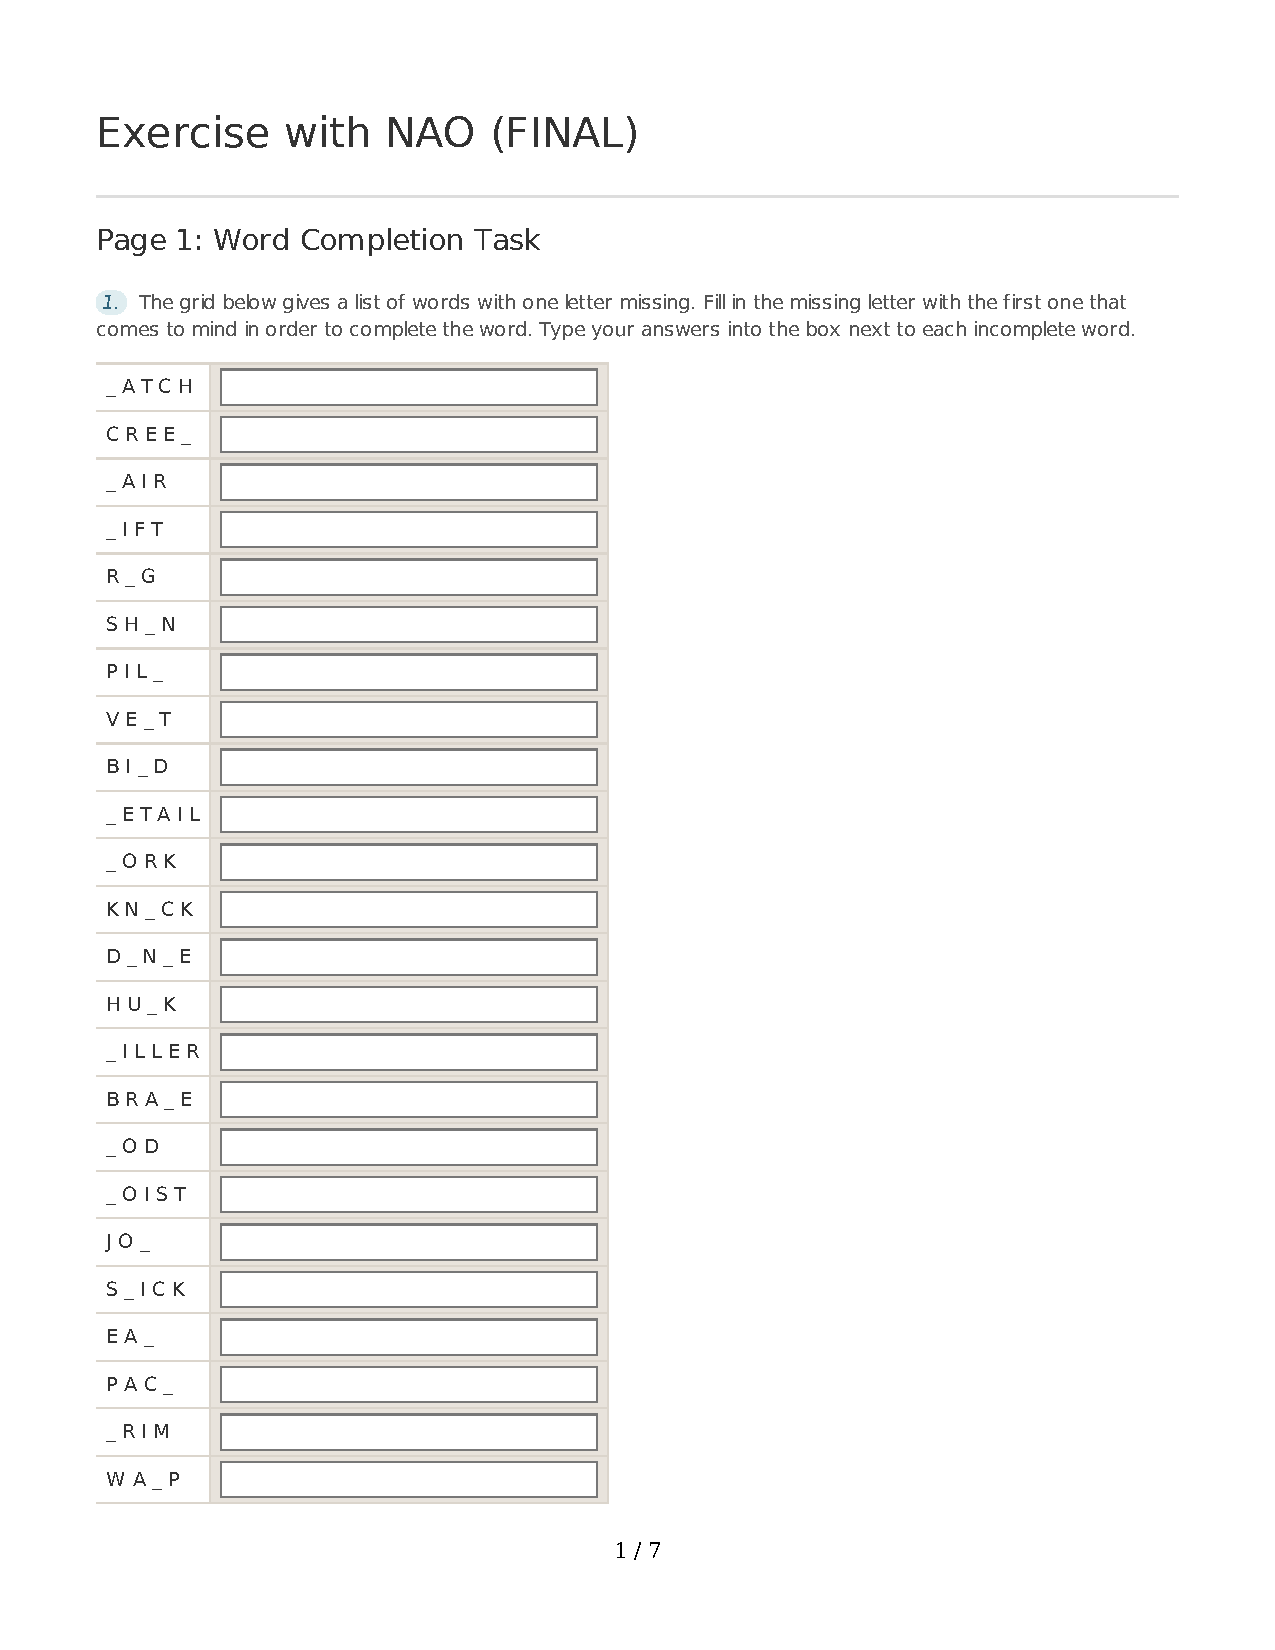
\includepdf[pages={-}]{Survey}

\end{document}